\documentclass[preprint,compress,3p,10pt,fleqn]{elsarticle}
%\usepackage{lineno,hyperref}
%\modulolinenumbers[5]
\usepackage{amscd}
\usepackage{amssymb}
\usepackage{amsmath}
\usepackage{bm}
\usepackage{subfigure}
\usepackage{color}
\usepackage{xcolor}
\usepackage{mathrsfs}
\usepackage{epsfig}
\usepackage{booktabs}
\usepackage{float}
\usepackage{ragged2e}
\usepackage{booktabs,makecell, multirow, tabularx}
%% cross reference jump
\usepackage{hyperref}
\hypersetup{
colorlinks=true,
linkcolor=black
}
\numberwithin{equation}{section}
%\numberwithin{table}{section}
%\numberwithin{figure}{section}
\newtheorem{theorem}{Theorem}[section]
\newtheorem{lemma}[theorem]{Lemma}
\newtheorem{remark}[theorem]{Remark}
% \newtheorem{lemma}{Lemma}[section]
% \newtheorem{remark}{Remark}[section]
\newtheorem{expl}{Example}[section]
\newenvironment{example}{\begin{expl}\rm}{\end{expl}}

\def\proof{\par{\it Proof}. \ignorespaces}
\def\endproof{\vbox{\hrule height0.6pt\hbox{%
\vrule height1.3ex width0.6pt\hskip0.8ex \vrule width0.6pt} \hrule
height0.6pt } \bigskip}

\renewcommand{\figurename}{Fig.}

%\journal{Journal of Appl. Math. Comput.}

% \bibliographystyle{elsarticle-num}

\begin{document}

\begin{frontmatter}

\title{Arbitrarily High-Order Explicit Energy-Conserving Methods for the Generalized Nonlinear Fractional Schr{\"o}dinger Wave Equations}
\author[myaddress]{Yang Liu}
\ead{liuyang@stu.sicnu.edu.cn}

\author[myaddress,mysecondaddress]{Maohua Ran\corref{mycorrespondingauthor}}
\cortext[mycorrespondingauthor]{Corresponding author.}
\ead{maohuaran@163.com}


%\author[mysecondaddress]{Li Zhang}
%\ead{lizhang−hit@163.com}

\address[myaddress]{School of Mathematical Sciences and V.C. and V.R. Key Lab, Sichuan Normal University, Chengdu 610068, China}
%\address[mysecondaddress]{V.C. and V.R. Key Lab of Sichuan Province, Sichuan Normal University, Chengdu 610068, China}
\address[mysecondaddress]{School of Mathematics, Aba Teachers University, Aba 623002, China}


\begin{abstract}
A novel category of explicit conservative numerical methods with arbitrarily high-order is introduced
for solving the nonlinear fractional Schr{\"o}dinger wave equations in one and two dimensions.
The proposed method is based on the scalar auxiliary variable approach. The equations studied is first
transformed into an equivalent system by introducing a scalar auxiliary variable, and the energy is
then reformulated as a sum of three quadratic terms. Applying the explicit
relaxation Runge-Kutta methods in temporal and the Fourier pseudo-spectral discretization in spatial,	the resulting time-space
full discrete scheme is proved to preserve the reformulated energy in the discrete level to machine
accuracy. The proposed methods improve the numerical stability during long-term computations, as demonstrated through numerical experiments.
Also this idea can be easily extended to other similar equations, such as the nonlinear
fractional  wave equation and the fractional Klein-Gordon-Schr{\"o}dinger equation.
\end{abstract}
	
\begin{keyword}
Structure-preserving method; Fractional Schr{\"o}dinger wave equations; Explicit relaxation Runge-Kutta method; Scalar auxiliary variable approach; Fourier pseudo-spectral method
\end{keyword}
	
\end{frontmatter}
	

	
	
\section{Introduction}\label{Section 1}
This paper focus on the numerical solution of the initial boundary-value problems of the nonlinear
fractional Schr{\"o}dinger wave equations (NFSWEs) as follows
\begin{align}
	&  u_{t t}+(-\Delta)^{\alpha / 2} u+\mathrm{i} \kappa u_{t}+\beta g(|u|^{2}) u=0, \quad \boldsymbol{x} \in \Omega, \quad  t \in(0, T],\label{eq_1}\\
& u(\boldsymbol{x}, 0)=u_{0}(\boldsymbol{x}), \quad u_{t}(\boldsymbol{x}, 0)=u_{1}(\boldsymbol{x}),\quad \boldsymbol{x} \in \Omega, \label{eq_2}\\
& u(\boldsymbol{x}+\boldsymbol{L}, t)=u(\boldsymbol{x}, t), \quad t \in[0, T],\label{eq_3}
\end{align}
where, $\mathrm{i}=\sqrt{-1}, 1<\alpha \leq 2$, and $\kappa, \beta(>0)$ are two real constants,
$ u(\boldsymbol{x}, t)$ is unknown complex valued function, $u_{0}(\boldsymbol{x})$ and
$u_{1}(\boldsymbol{x})$ are known smooth functions, the nonlinear term $g$ is a given real function,$\boldsymbol{x}\in\Omega\!\subset\!
R^d~(d\!=\!1,2)$ and $\boldsymbol{L}$ is the period. The fractional Laplacian operator can be expressed
in terms of the Fourier transform, as

\begin{align}\label{eq_4}
(-\Delta)^{\frac{\alpha}{2}} u(\boldsymbol{x},t)=\mathcal{F}^{-1}\left[|\boldsymbol{\xi}|^{\alpha} \mathcal{F}(u(\boldsymbol{\xi},t))\right],
\end{align}
where $\mathcal{F}$ and $\mathcal{F}^{-1}$ denote the Fourier transform and its inverse
respectively, see \cite{caffarelliExtensionProblemRelated2007}. The NFSWEs \eqref{eq_1}
can be considered as a generalization of the classical Schr{\"o}dinger wave
equations, the latter has numerous physical applications such as the Langmuir wave envelope
approximation in plasma \cite{colinSemidiscretizationTimeNonlinear1998}, and has been
studied in depth, see e.g., \cite{zhangConservativeNumericalScheme2003,baoUniformErrorEstimates2012,chengSeveralConservativeCompact2018,brugnanoClassEnergyconservingHamiltonian2018}.

Due to its importance in both theoretical and applied physics, there has been a great
deal of interest in developing efficient and accurate numerical methods for solving
the NFSWEs \eqref{eq_1}. Noticing that the NFSWEs has the following conservation law
of energy
\begin{align}\label{eq_9}
E(t)=\left\|u_{t}(\cdot, t)\right\|^{2}+\left\|(-\Delta)^{\frac{\alpha}{4}} u(\cdot, t)\right\|^{2}+\frac{\beta}{2} \int_{\mathbb{R}^d} G\left(|u|^2\right) d \boldsymbol{x}=E(0), \quad 0 \leq t \leq T,
\end{align}
where $G(s)=\int_0^s g(z) d z$, see \cite{baoUniformErrorEstimates2012,ranLinearlyImplicitConservative2016}.
The scholars have a more significant interest in structure-preserving methods.
This is because, for conservative problems, numerical methods that
can preserve the underlying invariance are usually advantageous. Besides, conservative
schemes can achieve good stability in long-time simulations. In the past few years, some
structure-preserving methods for the NFSWEs have been proposed. For instance, Ran and
Zhang \cite{ranLinearlyImplicitConservative2016} developed a three-level linearly implicit
difference scheme that preserves a modified discrete mass and energy.
Li and Zhao \cite{liFastEnergyConserving2018} proposed a conservative method by combing
the Crank-Nicolson method and the Galerkin finite element method. Moreover, a fast Krylov
subspace solver is introduced to reduce computational cost.
Cheng and Qin \cite{chengConvergenceEnergyconservingScheme2022} developed a linearly-implicit
conservative scheme based on the scalar auxiliary variable (SAV) method, which preserves only a modified energy,
but not mass. Hu et al. \cite{huEfficientEnergyPreserving2022} proposed three energy-preserving
spectral Galerkin methods by applying the Crank-Nicolson, SAV, and  exponential-SAV(ESAV) methods in time,
respectively. Zhang and Ran \cite{zhangHighorderStructurepreservingDifference2023} proposed and analyzed the higher order energy-preserving difference scheme based on triangular-SAV(T-SAV) approach. Nevertheless, most of these methods proposed in the above paper are only
focused on the one-dimensional case, have no higher than second-order accuracy in time,
and/or are fully-implicit. It means that there are still many open question, and efficient,
accurate and explicit numerical methods would be desirable for future investigations,
especially for high dimensions.	

Among the various numerical methods with high-order accuracy, explicit Runge-Kutta (RK) methods are good candidates,
because they belong to one-step methods, and have the characteristics of high
order accuracy and simplicity of implementation. However, the standard RK methods do not
necessarily preserve the desired physical properties of the system.  To overcome this issue,
Ketcheson \cite{ketchesonRelaxationRungeKutta2019} proposed the relaxation Runge-Kutta (RRK)
method, which guarantees conservation or stability with respect to any inner product norm.
Later, the RRK technique has been extended to general convex quantities in
\cite{ranochaRelaxationRungeKutta2020}. Hence, the conservation, dissipation, or other properties
with respect to any convex functional are enforced by the addition of a relaxation parameter
that multiplies the Runge-Kutta update at each step. The trade-off for these advantages is
that a nonlinear algebraic system has to be solved to determine the relaxation parameter.
Nevertheless, the construction of explicit conservative schemes for the case of non-quadratic
invariants has not been considered by the authors. Fortunately, the invariant energy
quadratization (IEQ) approach \cite{yangLinearUnconditionallyEnergy2017, yangEfficientLinearSchemes2017}
and the SAV approach \cite{chengConvergenceEnergyconservingScheme2022}
can transform the non-quadratic energy into a quadratic form of a new variable via a change of
variables, and the resulting new, equivalent system still retains a similar energy law in terms
of the new variables.
Motivated by these developments, this paper aims to develop numerical methods for the NFSWEs in one and two dimensions by combining the SAV method and the explicit RRK method.
And the proposed method has the following advantages:
\begin{itemize}
	\item explicit scheme;
	\item has accuracy of arbitrary high order in temporal direction;
	\item preserves the invariant quantity \eqref{eq_9}.
\end{itemize}

% Motivated by these developments, this paper aims to develop explicit
% numerical methods for the NFSWEs in one and two dimensions by combining the SAV method and the
% explicit RRK method.
% {\color{blue}These proposed explicit methods are expected to preserve the invariant quantity \eqref{eq_9} exactly at the discrete level, and have an arbitrary order of temporal accuracy.}

The remainder of this work is organized as follows. In Section \ref{Section 2}, we reformulate
the NFSWEs \eqref{eq_1} into an equivalent system by introducing a scalar auxiliary variable. Section
\ref{Section 3} obtains a semi-discrete conservative system by applying the Fourier pseudo-spectral
approximation to the resulting reformulation. In Section \ref{Section 4}, we present the explicit
fully-discrete schemes for the reformulated semi-discrete systems by applying the relaxation
Runge-Kutta method in time, and the proposed scalar auxiliary variable relaxation Runge-Kutta(SAV-RRK) schemes preserve the same convergence order
as the standard scalar auxiliary variable Runge-Kutta (SAV-RK) method. We further estimate the
relaxation coefficient introduced and then obtain the accuracy of the relaxation methods in
Section \ref{Section 5}. Numerical examples are presented in Section \ref{Section 6} to demonstrate
the accuracy and conservation properties of the proposed schemes. A  brief conclusion is drawn in
Section \ref{Section 7}.
	
\section{SAV reformulations of the NFSWEs}\label{Section 2}
	
It is well-known that all RK methods preserve arbitrary linear invariants, and only symplectic RK methods preserve arbitrary quadratic invariants. However, no RK methods can preserve arbitrary polynomial invariants of a degree higher than two or non-polynomial nonlinear invariants. To overcome this limitation and take advantage of the quadratic invariant-preserving property of relaxation RK methods, we adopt the newly developed SAV approach to rewrite high-degree energy functions as quadratic ones.
It allows the NFSWEs \eqref{eq_1} to be reformulated in equivalent forms that admit quadratic energy functions.
	
In order to maintain the positivity of the energy, we modify the energy in \eqref{eq_9} by adding a positive constant $C_0$ to $\frac{\beta}{2} \int_{\mathbb{R}^d} G\left(|u|^2\right) d \boldsymbol{x}$. This modification has no essential effect on the energy invariance of the system described in \eqref{eq_9}. Thus we will continue to use $E(t)$ for the modified energy, i.e.,
\begin{align}\label{eq_9_1}
E(t)\overset{\text{def}}{=}\left\|u_{t}(\cdot, t)\right\|^{2}+\left\|(-\Delta)^{\frac{\alpha}{4}} u(\cdot, t)\right\|^{2}+\frac{\beta}{2} \int_{\mathbb{R}^d} G\left(|u|^2\right) d \boldsymbol{x} + C_0.
\end{align}
In this, we consider a new scalar variable
\begin{equation}
w(t)\overset{\text{def}}{=}\sqrt{H(t)+C_0} \text { with } H(t)\overset{\text{def}}{=}\frac{\beta}{2} \int_{\Omega} G\left(|u|^2\right) d \boldsymbol{x}=\frac{\beta}{2}\int_{\Omega} \int_0^{|u|^2} g(z) d z d \boldsymbol{x}.
\end{equation}
The direct calculation produces that
\begin{align}
w_t & =\frac{1}{2 \sqrt{H(t)+C_0}} \frac{d H(t)}{d t} \nonumber\\
& =\frac{1}{2 \sqrt{H(t)+C_0}} \frac{d}{d t} \int_{\Omega} G(|u|^2) d \boldsymbol{x} \nonumber\\
& =\frac{\beta}{\sqrt{H(t)+C_0}} \int_{\Omega} g(|u|^2) \Re\left(u \bar{u}_t\right) d \boldsymbol{x}\nonumber\\
& =\Re \int_{\Omega} \frac{\beta g(|u|^2) u \bar{u}_t}{\sqrt{H(t)+C_0}} d \boldsymbol{x} \nonumber\\
& =\Re\left(b(u), u_t\right), \label{eq:2-1}
\end{align}
where
\begin{align}
b(u)\overset{\text{def}}{=}\beta g(|u|^2) u / \sqrt{H(t)+C_0},
\end{align}
$\Re$ denotes the real part and $(\cdot, \cdot)$ means the $L^2$-inner product over $\Omega$.
	
As a result, the NFSWEs \eqref{eq_1}-\eqref{eq_3} can be equivalently rewritten as
\begin{align}
& u_t=v, \label{eq:2-2}\\
& v_t=-(-\Delta)^{\alpha / 2} u-\mathrm{i}\kappa v-b(u) w, \label{eq:2-3}\\
& w_t=\Re\left(b(u), u_t\right),\label{eq:2-4}
\end{align}
with the initial conditions
\begin{align}\label{eq_31}
u(\boldsymbol{x}, 0)=u_{0}(\boldsymbol{x}), \quad v(\boldsymbol{x}, 0)=u_{1}(\boldsymbol{x}), \quad w(0)=\sqrt{\frac{\beta}{2} \int_{\mathbb{R}^d} G\left(|u_{0}|^2\right) d \boldsymbol{x} +C_0}.
\end{align}
	
Taking the inner product of systems \eqref{eq:2-2}-\eqref{eq:2-3} respectively with $v_t$ and $u_t$, multiplying \eqref{eq:2-4} by $w(t)$, summing the resulting equations, and finally taking a integration over the time interval $[0, t]$ for the real part, one immediately has the modified energy conservation law
\begin{equation}
E(t)=\|v(\cdot, t)\|^2+\left\|(-\Delta)^{\frac{\alpha}{4}} u(\cdot, t)\right\|^{2}+w^2(t)=E(0),
\end{equation}
which is essentially consistent with the original energy-conservation law \eqref{eq_9} for NFSWEs \eqref{eq_1}-\eqref{eq_3}.

	
\section{Structure-preserving spatial discretization}\label{Section 3}
Without loss of generality, we assume that the spatial dimension is two (i.e., $d=2$). The Fourier
pseudo-spectral method is a well-established technique for solving partial differential equations
that can provide accurate and efficient approximations. This method involves approximating the
solution in the spectral domain, where the derivatives are computed using fast Fourier transforms. Therefore, we utilize the Fourier pseudo-spectral method for the spatial discretization of the equivalent systems \eqref{eq:2-2}-\eqref{eq_31}.
	
For positive integer $M$ and even positive integers $N_{x}$ and $N_{y}$, denote $\tau\!=\!{T}/{M}, h_{x}\!=\!{L}/{N_{x}}, h_{y}\!=\!{L}/{N_{y}}$. Define $\Omega_{h}\!=\!\left\{\left(x_{i}, y_{j}\right) \mid 0 \leq i \leq N_x-1;0 \leq j \leq N_y-1\right\}, \Omega_{\tau}\!=\!\left\{t_{m} \mid 0 \leq m \leq M\right\}$ and $\Omega_{h}^{\tau}\!=\!\Omega_{h} \times \Omega_{\tau}$, with $t_{m}=m \tau, x_{i}=i h_{x}$ and $y_{j}=j h_{y}$.
The vector forms at any time level $t_m$ are given by
\begin{align}\label{eq_47}
&U^m=\left(u_{0,0}^m, \cdots, u_{N_{x}-1,0}^m, u_{0,1}^m, \cdots, u_{N_{x}-1,1}^m, \cdots, u_{0, N_{y}-1}^m, \cdots, u_{N_{x}-1, N_{y}-1}^m\right)^{T},\\
&V^m=\left(v_{0,0}^m, \cdots, v_{N_{x}-1,0}^m, v_{0,1}^m, \cdots, v_{N_{x}-1,1}^m, \cdots, v_{0, N_{y}-1}^m, \cdots, v_{N_{x}-1, N_{y}-1}^m\right)^{T},\\
&W^m=w^m.
\end{align}

For any grid functions $u$ and $v$ defined on $\Omega_{h}$, we define the discrete inner product and the associated discrete norms as
\begin{align}\label{eq_48}
(u, v)=h_{x} h_{y} \sum_{i=0}^{N_{x}-1} \sum_{j=0}^{N_{y}-1} u_{i, j} \bar{v}_{i, j}, \quad\|u\|=(u, u)^{\frac{1}{2}}, \quad\|u\|_{\infty}=\sup _{\left(x_{i}, y_{j}\right) \in \Omega_{h}}\left|u_{i, j}\right|.
\end{align}
	
Let $\left(x_{i}, y_{j}\right) \in \Omega_{h}$ be the Fourier collocation points. Denote $u_{N}(x, y)$ is the interpolation polynomial function of $u(x, y)$, then we have
\begin{align}\label{eq_50}
u_{N}(x, y)=\sum_{k_{1}=-N_{x} / 2}^{N_{x} / 2} \sum_{k_{2}=-N_{y} / 2}^{N_{y} / 2} \tilde{u}_{k_{1}, k_{2}} e^{\mathrm{i}\mu\left( k_{1} (x+L)+k_{2}(y+L)\right)},
\end{align}
in which $\mu={\pi}/{L}$, and the coefficients
\begin{align}\label{eq_51}
\tilde{u}_{k_{1}, k_{2}}=\frac{1}{N_{x} c_{k_{1}}} \frac{1}{N_{y} c_{k_{2}}} \sum_{l_1=0}^{N_{x}-1} \sum_{l_2=0}^{N_{y}-1} u(x_{l_1}, y_{l_2}) e^{-\mathrm{i}\mu\left( k_{1}(x_{l_1}+L)+k_{2}(y_{l_2}+L)\right)},
\end{align}
where $c_{k_{1}}=1$ for $\left|k_{1}\right|<N_{x}/2, c_{k_{2}}=1$ for $\left|k_{2}\right|<N_{y}/2, c_{k_{1}}=2$ for $k_{1}=\pm N_{x}/2$, and $c_{k_{2}}=2$ for $k_{2}=\pm N_{y}/2$.
	
As a result, the fractional Laplacian $(-\Delta)^{\frac{\alpha}{2}} u(x, y)$ can be approximated by
\begin{align}\label{eq_52}
(-\Delta)^{\frac{\alpha}{2}} u_{N}\left(x, y\right)=\sum\limits_{k_{1}=-N_{x} / 2}^{N_{x} / 2} \sum\limits_{k_{2}=-N_{y} / 2}^{N_{y} / 2}\left|\left(k_{1} \mu\right)^{2}+\left(k_{2} \mu\right)^{2}\right|^{\frac{\alpha}{2}} \tilde{u}_{k_{1}, k_{2}} e^{\mathrm{i}\mu\left( k_{1} (x+L)+k_{2}(y+L)\right)}.
\end{align}
Inserting \eqref{eq_51} into \eqref{eq_52}, and considering the resulting equation at the point $(x_i,y_j)$ gives that
\begin{align}
&(-\Delta)^{\frac{\alpha}{2}} u_{N}\left(x_{i}, y_{j}\right)\nonumber\\
=&\sum\limits_{l_{1}=0}^{N_{x}-1} \sum\limits_{l_{2}=0}^{N_{y}-1}u(x_{l_{1}}, y_{l_{2}})\Big(\sum\limits_{k_{1}=-N_{x} / 2}^{N_{x} / 2} \sum\limits_{k_{2}=-N_{y} / 2}^{N_{y} / 2} \frac{1}{N_{x} c_{k_{1}}} \frac{1}{N_{y} c_{k_{2}}}\left|\mu^{2} \cdot \mathbf{k}^{2}\right|^{\frac{\alpha}{2}} e^{\mathrm{i} \mu\left(k_{1}\left(x_{i}-x_{l_{1}}\right)+k_{2}\left(y_{j}-y_{l_{2}}\right)\right)}\Big)\nonumber\\
=&\left(D^{\alpha}U\right)_{i+j N_{x}},\label{eq_53}
\end{align}
where $\mu^{2} \cdot \mathbf{k}^{2}=\mu^{2}\left(k_{1}^{2}+k_{2}^{2}\right)$, $D^{\alpha}$ is spectral symmetric differential matrix with the elements
\begin{align}\label{eq_54}
\left(D^{\alpha}\right)_{i+j N_{x}, l_{1}+l_{2} N_{x}}=\sum\limits_{l_{1}=0}^{N_{x}-1} \sum\limits_{l_{2}=0}^{N_{y}-1}\frac{1}{N_{x} c_{k_{1}}} \frac{1}{N_{y} c_{k_{2}}}\left|\mu^{2} \cdot \mathbf{k}^{2}\right|^{\frac{\alpha}{2}} e^{\mathrm{i}\mu\left(k_{1}\left(x_{i}-x_{l_{1}}\right)+k_{2}\left(y_{j}-y_{l_{2}}\right)\right)}.
\end{align}
	
Above all, applying the Fourier pseudo-spectral method to the previous equivalent system \eqref{eq:2-2}-\eqref{eq:2-4} in space gives the semi-discrete system as follows
\begin{align}
& U_t=V, \label{eq:3-9}\\
& V_t=D^{\alpha} U-\mathrm{i}\kappa V- b(U) \cdot W, \label{eq:3-10}\\
& W_t=\Re\left(b(U), U_t\right),\label{eq:3-11}
\end{align}
with the initial conditions $U^0, V^0, W^0$, where $\cdot$ means the point multiplication between vectors.
	
For the semi-discrete system \eqref{eq:3-9}-\eqref{eq:3-11}, we have the following theorem.
\begin{theorem}	\label{thm3}
The space semi-discrete system \eqref{eq:3-9}-\eqref{eq:3-11} admits the semi-discrete quadratic energy conservation law
\begin{equation}
\frac{dE}{dt}=0, \label{eq:313a}
\end{equation}
where
\begin{equation}
E(U,V,W)\overset{\text{def}}{=}\|V\|^2 + \|D^\frac{\alpha}{2} U\|^2+\left(W\right)^2.\label{eq:313}
\end{equation}
\end{theorem}

\begin{proof}
	Taking the inner product of \eqref{eq:3-9}, \eqref{eq:3-10} with $V_t$ and $U_t$ respectively, and multiplying \eqref{eq:3-11} by $W$, we get
\begin{align}
&\left(V_t, U_t\right)=\left(V_t, V\right), \label{eq:313a}\\
&\left(V_t, U_t\right)=\left(D^{\alpha} U, U_t\right)-\mathrm{i} \kappa\left(V, U_t\right)-W\left(b(U), U_t\right), \label{eq:313b}\\
&W W_t=W\Re\left(b(U), U_t\right).\label{eq:313c}
\end{align}
Summing the resulting equations \eqref{eq:313a}-\eqref{eq:313c}, we have
\begin{equation}
\left(V_t, V\right) + W W_t= \left(D^{\alpha} U, U_t\right)-\mathrm{i} \kappa\left(V, U_t\right)-W\left(b(U), U_t\right) + W\Re\left(b(U), U_t\right).
\end{equation}
Taking the real part in above equation gives
\begin{align}
\Re\left(V_t, V\right) + \Re\left(W W_t\right)&= \Re\left(D^{\alpha} U, U_t\right)-\Re\left(\mathrm{i} \kappa\left(V, U_t\right)\right)-W\Re\left(b(U), U_t\right) + W\Re\left(b(U). U_t\right).
\end{align}
Thus, we know that
\begin{align}
\Re\left(V_t, V\right) + \Re\left(W W_t\right)&= \Re\left(D^{\alpha} U, U_t\right).\label{eq:319}
\end{align}
Noticing that
\begin{equation}
\Re\left(V_t, V\right) = \frac{1}{2}\frac{d }{d t}\|V\|^2, \quad \Re\left(W W_t\right) = \frac{1}{2}\frac{d }{d t}\left(W\right)^2,\quad \Re\left(D^{\alpha} U, U_t\right)=-\frac{1}{2}\frac{d }{d t}\|D^\frac{\alpha}{2}U\|^2,\label{eq:320}
\end{equation}
and substituting \eqref{eq:320} into \eqref{eq:319} leads to
\begin{equation}
\frac{d }{d t}\left(\|V\|^2+\|D^\frac{\alpha}{2}U\|^2+\left(W\right)^2\right)=0.
\end{equation}
This completes the proof.
\end{proof}

\section{Conservative explicit SAV-RRK methods}\label{Section 4}
This section is devoted to present the invariant-conserving explicit RRK methods for the NFSWEs based on the SAV approach.
We begin by recalling RRK methods and discussing their structure-preserving properties.

\subsection{Explicit SAV-RRK schemes}
For brevity, we introduce following symbols
\begin{equation}
\bm{y}=\left(U,V,W\right)^T,\bm{y}_0=\left(U^0,V^0,W^0\right)^T , \bm{f}=(f^1,f^2,f^3)^T\overset{\text{def}}{=}(V,D^{\alpha} U-\mathrm{i}\kappa V-b(U)\cdot W,\Re\left(b(U), U_t\right))^T.
\end{equation}
Then the semi-discrete system \eqref{eq:3-9}-\eqref{eq:3-11} based on SAV approach can be rewritten as
\begin{equation}
\left\{\begin{array}{l}
\bm{y}_t=\bm{f}(\bm{y}),\quad t \in(0, T],\\
\bm{y}(0)=\bm{y}_0.
\end{array}\right.\label{eq:3-121}
\end{equation}
	
Let $\bm{y}^m$  be the approximation to $\bm{y}\left(t_m\right)$. A $s$-stage explicit RK method \cite{hairerRungeKuttaMethods2015} applied to \eqref{eq:3-121} takes the form
\begin{equation}
\left\{\begin{array}{l}
\bm{Y}_{m i}=\bm{y}^m+\tau \sum\limits_{j=1}^{i-1} a_{i j} \bm{f}_{m j}, \quad i=1, \ldots, s, \\
\bm{y}^{m+1}=\bm{y}^m+\tau \sum\limits_{i=1}^s b_i \bm{f}_{m i},
\end{array}\right.\label{eq:4-31}
\end{equation}
where $\bm{f}_{m j}=\bm{f}\left(\bm{Y}_{m j}\right)$, $j=1, \ldots, s$. With the following notations
\begin{equation}
\begin{aligned}
A & =\left(a_{i j}\right)_{s \times s}, \quad a_{i j}=0 \quad \text { for } \quad j \geq i, \\
b & =\left(b_1, \cdots, b_s\right)^T,
\end{aligned}
\end{equation}
the $s$-stage explicit SAV-RK methods can be represented by a Butcher tableau
\begin{equation}
\begin{array}{c|c}
c & A \\
\hline \\
& b^T
\end{array}
\end{equation}
where the abscissa vectors $c=(c_1,c_2,\dots,c_s)$ satisfy $c_i=\sum\limits_{j=1}^s a_{i j}, i=1, \ldots, s$.
	
However, it is well known that only special implicit RK methods may be symplectic or algebraically stable, and there are no symplectic or algebraically stable explicit RK methods. This leads to the fact that the explicit SAV-RK methods fail to preserve the underlying conservation property of the original problem \eqref{eq:3-121}. Thus, we introduce the explicit SAV-RRK method. Concretely, consider a single step over the interval $\left[\hat{t}_m, \hat{t}_{m+1}\right], m \geq 0$, and let $\bm{y}_\gamma^m=\left(U^{m}_{\gamma},V^{m}_{\gamma},W^{m}_{\gamma}\right)^T$ be the numerical approximation to $\bm{y}\left(\hat{t}_m\right)$,
then a $s$-stage explicit SAV-RRK method for \eqref{eq:3-121} is defined as
\begin{equation}
\left\{\begin{array}{l}
\bm{Y}_{m i}=\bm{y}_\gamma^m+\tau \sum\limits_{j=1}^{i-1} a_{i j} \bm{f}_{m j}, \quad i=1, \ldots, s, \\
\bm{y}_\gamma^{m+1}=\bm{y}_\gamma^m+\gamma_m \tau \sum\limits_{i=1}^s b_i \bm{f}_{m i}.
\end{array}\right.\label{eq:4-3}
\end{equation}
Similarly, the $s$-stage RRK methods \eqref{eq:4-3} can be represented by a Butcher tableau
\begin{equation}
\begin{array}{c|c}
c & A \\
\hline \\
& \tilde{b}^T
\end{array}
\end{equation}
where $\tilde{b}=\gamma_m b$ and $\gamma_m\neq 0$ satisfies
\begin{equation}
\left\{\begin{array}{ll}
E_{\gamma}^{m+1}=E_{\gamma}^{m}, & if \quad  \sum\limits_{i=1}^s b_i \bm{f}_{m i} \neq 0,\\
\gamma_m=1, & if \quad  \sum\limits_{i=1}^s b_i \bm{f}_{m i} =0,
\end{array}\right.\label{eq:4-6}
\end{equation}
where
\begin{align}\label{eq:4-6b}
E_{\gamma}^{m}  =\|V_{\gamma}^{m}\|^2+\|D^\frac{\alpha}{2} U_{\gamma}^{m}\|^2+\big(W_{\gamma}^{m}\big)^2.
\end{align}

An outstanding advantage of the explicit SAV-RRK method \eqref{eq:4-3} is that one can calculate
explicitly the parameter $\gamma_m$. In fact, one know from \eqref{eq:4-6} that $\gamma_m=1$ for $\sum\limits_{i=1}^s b_i \bm{f}_{m i}=0$. When $\sum\limits_{i=1}^s b_i \bm{f}_{m i}\neq 0$, by a straightforward calculation one can get that
\begin{align}
E_{\gamma}^{m+1}  =&\|V_{\gamma}^{m+1}\|^2+\|D^\frac{\alpha}{2} U_{\gamma}^{m+1}\|^2+\big(W_{\gamma}^{m+1}\big)^2 \nonumber\\
=&\|V_{\gamma}^{m+1}\|^2- \big(U_{\gamma}^{m+1}, D^{\alpha} U_{\gamma}^{m+1}\big)+\big(W_{\gamma}^{m+1}\big)^2 \nonumber\\
=&\|V_{\gamma}^{m}+\gamma_m\tau\sum\limits_{i=1}^{s}b_if_{mi}^2\|^2 +\big(W_{\gamma}^{m}+\gamma_m\tau\sum\limits_{i=1}^{s}b_if_{mi}^3\big)^2\nonumber\\
&- \big(U_{\gamma}^{m}+\gamma_m\tau\sum\limits_{i=1}^{s}b_if_{mi}^1, D^{\alpha} \big(U_{\gamma}^{m}+\gamma_m\tau\sum\limits_{i=1}^{s}b_if_{mi}^1\big)\big)\nonumber\\
=&\|V_{\gamma}^{m}\|^2+\|D^\frac{\alpha}{2} U_{\gamma}^{m}\|^2+\big(W_{\gamma}^{m}\big)^2\nonumber\\ &+\big(V_{\gamma}^{m},\gamma_m\tau\sum\limits_{i=1}^{s}b_if_{mi}^2\big)+\big(\gamma_m\tau\sum\limits_{i=1}^{s}b_if_{mi}^2,V_{\gamma}^{m}\big)+\big\|\gamma_m\tau\sum\limits_{i=1}^{s}b_if_{mi}^2\big\|^2\nonumber\\
&- \big(U_{\gamma}^{m}, D^{\alpha} \big(\gamma_m\tau\sum\limits_{i=1}^{s}b_if_{mi}^1\big)\big)- \big(\gamma_m\tau\sum\limits_{i=1}^{s}b_if_{mi}^1, D^{\alpha}U_{\gamma}^{m}\big)\nonumber\\
&+ \big\|D^\frac{\alpha}{2}\big(\gamma_m\tau\sum\limits_{i=1}^{s}b_if_{mi}^1\big)\big\|^2+2W_{\gamma}^{m}\gamma_m\tau\sum\limits_{i=1}^{s}b_if_{mi}^3+\big(\gamma_m\tau\sum\limits_{i=1}^{s}b_if_{mi}^3\big)^2\nonumber\\
=& E_{\gamma}^{m}+\gamma_m\tau\big[\big(V_{\gamma}^{m},\sum\limits_{i=1}^{s}b_if_{mi}^2\big)+\big(\sum\limits_{i=1}^{s}b_if_{mi}^2,V_{\gamma}^{m}\big)\big.\nonumber\\
&\big.-\big(U_{\gamma}^{m},D^{\alpha} \big(\sum\limits_{i=1}^{s}b_if_{mi}^1\big)\big)-\big(\sum\limits_{i=1}^{s}b_if_{mi}^1, D^{\alpha} U_{\gamma}^{m}\big)+2W_{\gamma}^{m}\sum\limits_{i=1}^{s}b_if_{mi}^3\big]\nonumber\\
&+\gamma_m^2\tau^2\big[\big\|\sum\limits_{i=1}^{s}b_if_{mi}^2\big\|^2+ \big\|D^\frac{\alpha}{2}\big(\sum\limits_{i=1}^{s}b_if_{mi}^1\big)\big\|^2+\big(\sum\limits_{i=1}^{s}b_if_{mi}^3\big)^2\big].\label{eq:49}
\end{align}
This together with \eqref{eq:4-6} gives that
\begin{align*}
&\gamma_m\tau\big[\big(V_{\gamma}^{m},\sum\limits_{i=1}^{s}b_if_{mi}^2\big)+\big(\sum\limits_{i=1}^{s}b_if_{mi}^2,V_{\gamma}^{m}\big)-\big(U_{\gamma}^{m},D^{\alpha} \big(\sum\limits_{i=1}^{s}b_if_{mi}^1\big)\big)-\big(\sum\limits_{i=1}^{s}b_if_{mi}^1, D^{\alpha} U_{\gamma}^{m}\big)\big.\\
&\big.+2W_{\gamma}^{m}\sum\limits_{i=1}^{s}b_if_{mi}^3\big] +\gamma_m^2\tau^2\big[\big\|\sum\limits_{i=1}^{s}b_if_{mi}^2\big\|^2+ \big\|D^\frac{\alpha}{2}\big(\sum\limits_{i=1}^{s}b_if_{mi}^1\big)\big\|^2+\big(\sum\limits_{i=1}^{s}b_if_{mi}^3\big)^2\big]=0,
\end{align*}
which is a quadratic algebraic equation for $\gamma_m$. Noting that $\gamma_m \neq 0$, thus
\begin{equation}\label{eq:r1}
\gamma_m\!=\!\frac{\big(V_{\gamma}^{m},\sum\limits_{i=1}^{s}b_if_{mi}^2\big)\!+\!\big(\sum\limits_{i=1}^{s}b_if_{mi}^2,V_{\gamma}^{m}\big)\!-\!\big(U_{\gamma}^{m},
D^{\alpha}\!\big(\sum\limits_{i=1}^{s}b_if_{mi}^1\big)\big)\!-\!\big(\sum\limits_{i=1}^{s}b_if_{mi}^1, D^{\alpha} U_{\gamma}^{m}\big)\!+\!2W_{\gamma}^{m}\sum\limits_{i=1}^{s}b_if_{mi}^3}{-\tau\big[\big\|\sum\limits_{i=1}^{s}b_if_{mi}^2\big\|^2\!+ \! \big\|D^\frac{\alpha}{2}\big(\sum\limits_{i=1}^{s}b_if_{mi}^1\big)\big\|^2\!+\!\big(\sum\limits_{i=1}^{s}b_if_{mi}^3\big)^2\big]} .
\end{equation}
This means that the value of $\gamma_m$ can also be explicitly determine by \eqref{eq:r1} when $\sum\limits_{i=1}^s b_i \bm{f}_{m i}\neq 0$.
	
Actually, the value of $\gamma_m$ defined in \eqref{eq:4-6} is close to $1$ as $\tau\rightarrow 0$,
which will be further discussed in Section \ref{Section 5-1}. Therefore, the explicit SAV-RRK methods \eqref{eq:4-3} are well-defined. Moreover, it can be proved that the proposed methods preserve the energy invariance described in the following theorem.
\begin{theorem}
	Suppose the order of explicit SAV-RK methods \eqref{eq:4-31} is at least two, then the solution to explicit SAV-RRK methods \eqref{eq:4-3} satisfies
\begin{equation}
E_{\gamma}^{m+1}=E_{\gamma}^{m}, \label{eq:4-10}
\end{equation}
where $E_{\gamma}^{m}$ is fined by \eqref{eq:4-6b}.
\end{theorem}

\begin{proof}
When $\sum\limits_{i=1}^s b_i \bm{f}_{m i}=0$, it follows from the second equation in \eqref{eq:4-3} that $\bm{y}_\gamma^{m+1}\equiv\bm{y}_\gamma^m$, which automatically satisfies \eqref{eq:4-10}. For the case of $\sum\limits_{i=1}^s b_i \bm{f}_{m i}\neq 0$, we can also get \eqref{eq:4-10} from the condition \eqref{eq:4-6}. This proof is completed.
\end{proof}
	
\section{Accuracy of the explicit SAV-RRK methods}\label{Section 5}
In this section, we will discuss the accuracy of the explicit SAV-RRK methods \eqref{eq:4-3}. To this end, we first estimate the relaxation coefficient $\gamma_m$, which plays a key role in the next analysis.
Since the relaxation coefficient $\gamma_m$ tends to vary from step to step, it can be estimated in the similar way over different steps. From this, here we just consider a single step over the interval $\left[\hat{t}_m, \hat{t}_{m+1}\right]$.

\subsection{Estimate of the relaxation coefficient}\label{Section 5-1}

We will only focus on the case of $\sum\limits_{i=1}^s b_i \bm{f}_{m i} \neq 0$, because the converse is simple.

Let
\begin{equation}
\begin{aligned}\label{eq:sm}
S_m(\gamma)=&\big\|V_\gamma^m+\gamma \tau \sum\limits_{i=1}^s b_i \bm{f}_{m i}^2\big\|^2 + \big\|D^\frac{\alpha}{2} \big(U_\gamma^m+\gamma \tau \sum\limits_{i=1}^s b_i \bm{f}_{m i}^1\big)\big\|^2\\
&+\big(W_\gamma^m+\gamma \tau \sum\limits_{i=1}^s b_i \bm{f}_{m i}^3\big)^2-\|V_\gamma^{m}\|^2 - \|D^\frac{\alpha}{2} U_\gamma^{m}\|^2-\big(W_\gamma^{m}\big)^2,
\end{aligned}
\end{equation}
then the value of $\gamma_m$ defined in \eqref{eq:4-6} is exactly the nonzero root of the function $S_m(\gamma)$.

    Moreover, we have following results on $S_m(\gamma)$.
\begin{lemma}\label{lem:5_1}
Suppose the order of explicit SAV-RK methods \eqref{eq:4-31} is $p$, then it holds that
\begin{equation}
S_m(1)=\mathcal{O}(\tau^{p+1}).
\end{equation}
\end{lemma}

\begin{proof}
Similar to the proof of Lemma $3.1$ in \cite{liImplicitexplicitRelaxationRungeKutta2022}, we consider the initial value problem
\begin{equation}
\left\{\begin{array}{l}
\tilde{\bm{y}}^{\prime}=\bm{f}(\tilde{\bm{y}}), \quad t \geq \hat{t}_m, \\
\tilde{\bm{y}}\left(\hat{t}_m\right)=\bm{y}_\gamma^m,
\end{array}\right.
\end{equation}
where $\bm{y}_\gamma^m$ is the solution to explicit SAV-RRK methods \eqref{eq:4-3}. By performing a single step using the explicit SAV-RRK methods \eqref{eq:4-3}, we arrive at the numerical solution $\bm{y}_\gamma^{m+1}$. It follows from \eqref{eq:sm} that
\begin{equation}
\begin{aligned}
S_m(\gamma) =& \|V_\gamma^{m+1}\|^2 + \|D^\frac{\alpha}{2} U_\gamma^{m+1}\|^2+\big(W_\gamma^{m+1}\big)^2-\|V_\gamma^{m}\|^2 - \|D^\frac{\alpha}{2} U_\gamma^{m}\|^2-\big(W_\gamma^{m}\big)^2\\
=& \|V_\gamma^{m+1}\|^2 + \|D^\frac{\alpha}{2} U_\gamma^{m+1}\|^2+\big(W_\gamma^{m+1}\big)^2-\|\tilde{V}(\hat{t}_{m})\|^2 - \|D^\frac{\alpha}{2} \tilde{U}(\hat{t}_{m})\|^2-\big(\tilde{W}(\hat{t}_{m})\big)^2.
\end{aligned}
\end{equation}

From $\bm{y}_\gamma^m$, the explicit SAV-RK methods \eqref{eq:4-31} of order $p$ generates the numerical solution  $\tilde{\bm{y}}^{m+1}$, which satisfies $\tilde{\bm{y}}^{m+1}=\tilde{\bm{y}}\left(\hat{t}_m+\tau\right)+\mathcal{O}\left(\tau^{p+1}\right)$ for sufficiently small $\tau$. It is crucial to observe that the explicit SAV-RRK methods defined by \eqref{eq:4-3} will reduce to the explicit SAV-RK methods described by \eqref{eq:4-31} when $\gamma=1$. That is $\bm{y}_\gamma^{m +1}=\tilde{\bm{y}}^{m +1}$. Consequently, we can derive that
\begin{align}
S_m(1) = &\|\tilde{V}^{m+1}\|^2 + \|D^\frac{\alpha}{2} \tilde{U}^{m+1}\|^2+\big(\tilde{W}^{m+1}\big)^2-\|\tilde{V}(\hat{t}_{m})\|^2 - \|D^\frac{\alpha}{2} \tilde{U}(\hat{t}_{m})\|^2-\big(\tilde{W}(\hat{t}_{m})\big)^2 \nonumber\\
= &\|\tilde{V}^{m+1}\|^2 -\|\tilde{V}(\hat{t}_{m}+\tau)\|^2 +\|\tilde{V}(\hat{t}_{m}+\tau)\|^2-\|\tilde{V}(\hat{t}_{m})\|^2\nonumber\\
& + \|D^\frac{\alpha}{2} \tilde{U}^{m+1}\|^2 -\|D^\frac{\alpha}{2} \tilde{U}(\hat{t}_{m}+\tau)\|^2+\|D^\frac{\alpha}{2} \tilde{U}(\hat{t}_{m}+\tau)\|^2- \|D^\frac{\alpha}{2} \tilde{U}(\hat{t}_{m})\|^2\nonumber\\
& +\big(\tilde{W}^{m+1}\big)^2 -\big(\tilde{W}(\hat{t}_{m}+\tau)\big)^2+\big(\tilde{W}(\hat{t}_{m}+\tau)\big)^2-\big(\tilde{W}(\hat{t}_{m})\big)^2 \nonumber\\
= &\mathcal{O}\big(\tau^{p+1}\big) +2\int_{\hat{t}_m}^{\hat{t}_m+\tau}\big[\Re\big(V_t, V\big) + \Re\big(W W_t\big) - \Re\big(D^{\alpha} U, U_t\big)\big]dt.\label{eq:54}
\end{align}
By combining \eqref{eq:54} and \eqref{eq:319}, this proof is complete.
\end{proof}
	
% \begin{lemma}\label{lem:5_2}
% Suppose the order of explicit SAV-RK methods \eqref{eq:4-31} is at least two, it holds
% \begin{equation}
% S_m^{\prime}(0)=\tilde{c} \tau+\mathcal{O}(\tau^2),~~S_m^{\prime}(1)=\tilde{c} \tau+\mathcal{O}(\tau^2)
% \end{equation}
% where $\tilde{c}$ is a constant.
% \end{lemma}

% \begin{proof}
% According the definition of $S_m(\gamma)$ in \eqref{eq:sm}, it follows from\eqref{eq:49} that
% \begin{align}\label{eq:5_4a}
% S_m(\gamma)=&E_{\gamma}^{m+1}-E_{\gamma}^{m}\nonumber\\
% =&\gamma\tau\Big[(V_{\gamma}^{m},\sum\limits_{i=1}^{s}b_if_{mi}^2)+(\sum\limits_{i=1}^{s}b_if_{mi}^2,V_{\gamma}^{m})-(U_{\gamma}^{m},D^{\alpha} (\sum\limits_{i=1}^{s}b_if_{mi}^1))-(\sum\limits_{i=1}^{s}b_if_{mi}^1, D^{\alpha} U_{\gamma}^{m})\nonumber\\
% &+2W_{\gamma}^{m}\sum\limits_{i=1}^{s}b_if_{mi}^3\Big]+\gamma^2\tau^2\Big[\|\sum\limits_{i=1}^{s}b_if_{mi}^2\|^2+ \|D^\frac{\alpha}{2}(\sum\limits_{i=1}^{s}b_if_{mi}^1)\|^2+(\sum\limits_{i=1}^{s}b_if_{mi}^3)^2\Big].
% \end{align}
% A straightforward calculation gives that
% \begin{align}\label{eq:5_4b}
% S_m^{\prime}(\gamma)=&\tau\Big[(V_{\gamma}^{m},\sum\limits_{i=1}^{s}b_if_{mi}^2)+(\sum\limits_{i=1}^{s}b_if_{mi}^2,V_{\gamma}^{m})-(U_{\gamma}^{m},D^{\alpha} (\sum\limits_{i=1}^{s}b_if_{mi}^1))-(\sum\limits_{i=1}^{s}b_if_{mi}^1, D^{\alpha} U_{\gamma}^{m})\nonumber\\
% &+2W_{\gamma}^{m}\sum\limits_{i=1}^{s}b_if_{mi}^3\Big]+2\gamma\tau^2\Big[\|\sum\limits_{i=1}^{s}b_if_{mi}^2\|^2+ \|D^\frac{\alpha}{2}(\sum\limits_{i=1}^{s}b_if_{mi}^1)\|^2+(\sum\limits_{i=1}^{s}b_if_{mi}^3)^2\Big].
% \end{align}
% Denote $\tilde{\bm{f}}_m=\bm{f}\left(\bm{y}\left(\tilde{t}_m\right)\right)$, then we have $\bm{f}_{m i}=\tilde{\bm{f}}_m+\mathcal{O}(\tau)$ as $\tau\rightarrow 0$.
% Thus, it holds that
% \begin{align*}			S_m^{\prime}(0)=&\tau\Big[(V_{\gamma}^{m},\sum\limits_{i=1}^{s}b_i\tilde{f}_{mi}^2)+(\sum\limits_{i=1}^{s}b_i\tilde{f}_{mi}^2,V_{\gamma}^{m})-(U_{\gamma}^{m},D^{\alpha} (\sum\limits_{i=1}^{s}b_i\tilde{f}_{mi}^1))-(\sum\limits_{i=1}^{s}b_i\tilde{f}_{mi}^1, D^{\alpha} U_{\gamma}^{m})\\
% &+2W_{\gamma}^{m}\sum\limits_{i=1}^{s}b_i\tilde{f}_{mi}^3\Big]+\mathcal{O}(\tau^2)\\
% =&\tilde{c}\tau+\mathcal{O}(\tau^2),
% \end{align*}
% and
% \begin{align*}	S_m^{\prime}(1)=&\tau\Big[(V_{\gamma}^{m},\sum\limits_{i=1}^{s}b_i\tilde{f}_{mi}^2)+(\sum\limits_{i=1}^{s}b_i\tilde{f}_{mi}^2,V_{\gamma}^{m})-(U_{\gamma}^{m},D^{\alpha} (\sum\limits_{i=1}^{s}b_i\tilde{f}_{mi}^1))-(\sum\limits_{i=1}^{s}b_i\tilde{f}_{mi}^1, D^{\alpha} U_{\gamma}^{m})\\
% &+2W_{\gamma}^{m}\sum\limits_{i=1}^{s}b_i\tilde{f}_{mi}^3\Big]+2\tau^2\Big[\|\sum\limits_{i=1}^{s}b_i\tilde{f}_{mi}^2\|^2+ \|D^\frac{\alpha}{2}(\sum\limits_{i=1}^{s}b_i\tilde{f}_{mi}^1)\|^2+(\sum\limits_{i=1}^{s}b_i\tilde{f}_{mi}^3)^2\Big]+\mathcal{O}(\tau^2)\\
% =&\tilde{c}\tau+\mathcal{O}(\tau^2).
% \end{align*}
% where
% \begin{align*} &\tilde{c}\!\overset{\text{def}}{=}\!(V_{\gamma}^{m},\sum\limits_{i=1}^{s}b_i\tilde{f}_{mi}^2)\!+\!(\sum\limits_{i=1}^{s}b_i\tilde{f}_{mi}^2,V_{\gamma}^{m})\!-\!(U_{\gamma}^{m},D^{\alpha} (\sum\limits_{i=1}^{s}b_i\tilde{f}_{mi}^1))\!-\!(\sum\limits_{i=1}^{s}b_i\tilde{f}_{mi}^1, D^{\alpha} U_{\gamma}^{m})\!+\!2W_{\gamma}^{m}\!\sum\limits_{i=1}^{s}b_i\tilde{f}_{mi}^3.
% \end{align*}
% This completes the proof.
% \end{proof}

% Based on Lemmas \ref{lem:5_1} and \ref{lem:5_2}, we can get the following estimation for the relaxation coefficient $\gamma_m$.
% \begin{theorem}\label{thm:5_1}
% Suppose the order of explicit SAV-RK methods \eqref{eq:4-31} is $p~(p \geq 2)$, then the relaxation coefficient $\gamma_m$ defined in \eqref{eq:4-6} satisfies
% \begin{equation}\label{eq:5_3}
% \gamma_m=1+\mathcal{O}(\tau^{p-1}).
% \end{equation}
% \end{theorem}

% \begin{proof}
% When $\sum\limits_{i=1}^s b_i \bm{f}_{m i}=0$, it follows from \eqref{eq:4-6} that $\gamma_m=1$, which automatically satisfies \eqref{eq:5_3}.

% When $\sum\limits_{i=1}^s b_i \bm{f}_{m i}\neq 0$, it follows from \eqref{eq:5_4a} that
% \begin{align}\label{eq:5_4a1}
% S_m(\gamma)=a\gamma^2+b\gamma,~~S_m'(\gamma)=2a\gamma+b,
% \end{align}
% where
% \begin{align*}
% &a\overset{\text{def}}{=}\tau^2\big[\|\sum\limits_{i=1}^{s}b_if_{mi}^2\|^2+ \|D^\frac{\alpha}{2}(\sum\limits_{i=1}^{s}b_if_{mi}^1)\|^2+(\sum\limits_{i=1}^{s}b_if_{mi}^3)^2\big],\\
% &b\!\overset{\text{def}}{=}\!\tau\big[(V_{\gamma}^{m},\sum\limits_{i=1}^{s}b_if_{mi}^2)\!+\!(\sum\limits_{i=1}^{s}b_if_{mi}^2,V_{\gamma}^{m})\!-\!(U_{\gamma}^{m},D^{\alpha} (\sum\limits_{i=1}^{s}b_if_{mi}^1))\!-\!(\sum\limits_{i=1}^{s}b_if_{mi}^1, D^{\alpha} U_{\gamma}^{m})\!+\!2W_{\gamma}^{m}\sum\limits_{i=1}^{s}b_if_{mi}^3\big].
% \end{align*}
% This combining with Lemma \ref{lem:5_1} gives
% \begin{equation}\label{eq:5_4a2}
% 	S_m(1) =a + b =\mathcal{O}(\tau^{p+1}).
% \end{equation}
% Similarly, combining \eqref{eq:5_4a1} with Lemma \ref{lem:5_2}, we can deduce that
% \begin{equation}\label{eq:5_4a3}
% \left\{\begin{array}{l}
% S_m^{\prime}(0)=b=\tilde{c} \tau+\mathcal{O}(\tau^2), \\
% S_m^{\prime}(1)=2 a+b=\tilde{c} \tau+\mathcal{O}(\tau^2).
% \end{array}\right.	
% \end{equation}
% This implies that $a=\mathcal{O}(\tau^2)$.

% Noting that $S_m(\gamma)$ is a quadratic function of $\gamma$, thus the non-zero root
% \begin{align*}
% \gamma&=-\frac{b}{a}=-\frac{\mathcal{O}(\tau^{p+1})-a}{a}=1-\frac{\mathcal{O}(\tau^{p+1})}{a}=1-\frac{\mathcal{O}(\tau^{p+1})}{\mathcal{O}(\tau^2)}=1+\mathcal{O}(\tau^{p-1}) .
% \end{align*}
% This completes the proof.
% \end{proof}
Based on Lemma \ref{lem:5_1}, we can get the following estimation for the relaxation coefficient $\gamma_m$.
	
\begin{theorem}\label{thm:5_1}
	Suppose the order of explicit SAV-RK methods \eqref{eq:4-31} is $p~(p \geq 2)$, then the relaxation coefficient $\gamma_m$ defined in \eqref{eq:4-6} satisfies
	\begin{equation}\label{eq:5_3}
	\gamma_m=1+\mathcal{O}(\tau^{p-1}).
	\end{equation}
	\end{theorem}	
	
	\begin{proof}
	% When $\sum\limits_{i=1}^s b_i \bm{f}_{m i}=0$, it follows from \eqref{eq:4-6} that $\gamma_m=1$, which automatically satisfies \eqref{eq:5_3}.
	% When $\sum\limits_{i=1}^s b_i \bm{f}_{m i}\neq 0$, according the definition of $S_m(\gamma)$ in \eqref{eq:sm}, it follows from\eqref{eq:49} that
	Let us consider two cases based on the value of $\sum\limits_{i=1}^s b_i \bm{f}_{m i}$.

	Case 1: According the definition of $\gamma_m$ in \eqref{eq:4-6}, we have $\gamma_m = 1$ when $\sum\limits_{i=1}^s b_i \bm{f}_{m i} = 0$, which automatically satisfies \eqref{eq:5_3}.

	Case 2: When $\sum\limits_{i=1}^s b_i \bm{f}_{m i} \neq 0$, it follows from \eqref{eq:49} that
	\begin{align}\label{eq:5_4a}
	S_m(\gamma)=&~E_{\gamma}^{m+1}-E_{\gamma}^{m}\nonumber\\
	=&~\gamma\tau\Big[(V_{\gamma}^{m},\sum\limits_{i=1}^{s}b_if_{mi}^2)+(\sum\limits_{i=1}^{s}b_if_{mi}^2,V_{\gamma}^{m})-(U_{\gamma}^{m},D^{\alpha} (\sum\limits_{i=1}^{s}b_if_{mi}^1))-(\sum\limits_{i=1}^{s}b_if_{mi}^1, D^{\alpha} U_{\gamma}^{m})\nonumber\\
	&+2W_{\gamma}^{m}\sum\limits_{i=1}^{s}b_if_{mi}^3\Big]+\gamma^2\tau^2\Big[\|\sum\limits_{i=1}^{s}b_if_{mi}^2\|^2+ \|D^\frac{\alpha}{2}(\sum\limits_{i=1}^{s}b_if_{mi}^1)\|^2+(\sum\limits_{i=1}^{s}b_if_{mi}^3)^2\Big].
	\end{align}
	Noting that $S_m(\gamma)$ is a quadratic function of $\gamma$, it has non-zero root
	\begin{equation}\label{eq:5_4a3}
		\gamma=\!\frac{\tau\Big[(V_{\gamma}^{m},\sum\limits_{i=1}^{s}b_if_{mi}^2)\!+\!(\sum\limits_{i=1}^{s}b_if_{mi}^2,V_{\gamma}^{m})\!-\!(U_{\gamma}^{m},D^{\alpha} (\sum\limits_{i=1}^{s}b_if_{mi}^1))\!-\!(\sum\limits_{i=1}^{s}b_if_{mi}^1, D^{\alpha} U_{\gamma}^{m})\!+\!2W_{\gamma}^{m}\sum\limits_{i=1}^{s}b_if_{mi}^3\Big]}{-\tau^2\Big[\|\sum\limits_{i=1}^{s}b_if_{mi}^2\|^2\!+\! \|D^\frac{\alpha}{2}(\sum\limits_{i=1}^{s}b_if_{mi}^1)\|^2\!+\!(\sum\limits_{i=1}^{s}b_if_{mi}^3)^2\Big]}.
	\end{equation}
Based on Lemma \ref{lem:5_1}, we have
\begin{align}\label{eq:5_4a2}
	S_m(1)=&\tau\Big[(V_{\gamma}^{m},\sum\limits_{i=1}^{s}b_if_{mi}^2)+(\sum\limits_{i=1}^{s}b_if_{mi}^2,V_{\gamma}^{m})-(U_{\gamma}^{m},D^{\alpha} (\sum\limits_{i=1}^{s}b_if_{mi}^1))-(\sum\limits_{i=1}^{s}b_if_{mi}^1, D^{\alpha} U_{\gamma}^{m})\nonumber\\
	&+2W_{\gamma}^{m}\sum\limits_{i=1}^{s}b_if_{mi}^3\Big]+\tau^2\Big[\|\sum\limits_{i=1}^{s}b_if_{mi}^2\|^2+ \|D^\frac{\alpha}{2}(\sum\limits_{i=1}^{s}b_if_{mi}^1)\|^2+(\sum\limits_{i=1}^{s}b_if_{mi}^3)^2\Big]\nonumber\\
	=&\mathcal{O}(\tau^{p+1}).
	\end{align}
Defining $\tilde{\bm{f}}_m=\bm{f}\left(\bm{y}\left(\tilde{t}_m\right)\right)$, then we have $\bm{f}_{m i}=\tilde{\bm{f}}_m+\mathcal{O}(\tau)$ as $\tau\rightarrow 0$.
Thus, it holds that
\begin{align}\label{eq:5_4a4}
	&\tau^2\Big[\|\sum\limits_{i=1}^{s}b_if_{mi}^2\|^2+ \|D^\frac{\alpha}{2}(\sum\limits_{i=1}^{s}b_if_{mi}^1)\|^2+(\sum\limits_{i=1}^{s}b_if_{mi}^3)^2\Big]\nonumber\\
	=&\tau^2\Big[\|\sum\limits_{i=1}^{s}b_i\tilde{f}_{mi}^2\|^2+ \|D^\frac{\alpha}{2}(\sum\limits_{i=1}^{s}b_i\tilde{f}_{mi}^1)\|^2+(\sum\limits_{i=1}^{s}b_i\tilde{f}_{mi}^3)^2\Big]+\mathcal{O}(\tau^3)\nonumber\\
	=&\mathcal{O}(\tau^2).
	\end{align}
Substituting \eqref{eq:5_4a4} and \eqref{eq:5_4a2} into \eqref{eq:5_4a3} yields that
%Dividing both sides of \eqref{eq:5_4a2} by $-\tau^2\Big[\|\sum\limits_{i=1}^{s}b_if_{mi}^2\|^2+ \|D^\frac{\alpha}{2}(\sum\limits_{i=1}^{s}b_if_{mi}^1)\|^2+(\sum\limits_{i=1}^{s}b_if_{mi}^3)^2\Big]$ and utilizing \eqref{eq:5_4a4}, we have
\begin{align}\label{eq:5_4a5}
	\gamma&=1+\frac{\mathcal{O}(\tau^{p+1})}{-\tau^2\Big[\|\sum\limits_{i=1}^{s}b_if_{mi}^2\|^2+ \|D^\frac{\alpha}{2}(\sum\limits_{i=1}^{s}b_if_{mi}^1)\|^2+(\sum\limits_{i=1}^{s}b_if_{mi}^3)^2\Big]}\nonumber\\
	&=1+\frac{\mathcal{O}(\tau^{p+1})}{\mathcal{O}(\tau^2)}\nonumber\\
	&=1+\mathcal{O}(\tau^{p-1}).
	\end{align}
	This proof is completed.
	\end{proof}

\begin{remark}\label{rk:5_1}
Theorem \ref{thm:5_1} shows that the relaxation coefficient $\gamma_m$ is close to $1$ as $\tau\rightarrow 0$,
which implies that the relaxation methods can be considered as a small perturbation of the standard methods.
\end{remark}
	
\subsection{Truncation errors of the explicit SAV-RRK methods}
Now we further study the accuracy of the explicit SAV-RRK methods \eqref{eq:4-3} based on the estimates on the relaxation coefficient $\gamma_m$ given by Theorem \ref{thm:5_1}.
	
Before analyzing the accuracy of the methods, we rewrite the explicit SAV-RRK methods \eqref{eq:4-3} into
\begin{equation}
\left\{\begin{array}{l}
\bm{Y}_{m i}=\bm{y}_\gamma^m+\tau \sum\limits_{j=1}^{i-1} a_{i j} \bm{f}_{m j}, \quad i=1, \ldots, s, \\
\bm{y}^{m+1}=\bm{y}_\gamma^m+\tau \sum\limits_{i=1}^s b_i \bm{f}_{m i},\\
\bm{y}_\gamma^{m+1}=\bm{y}^{m+1}+\left(\gamma_m-1\right)\left(\bm{y}^{m+1}-\bm{y}_\gamma^m\right) .
\end{array}\right.\label{eq:4-321}
\end{equation}
The first two equations essentially form the standard explicit SAV-RK methods.

Similar to the discussion in \cite{ketchesonRelaxationRungeKutta2019}, the numerical solution $\bm{y}_\gamma^{m+1}$ at $\hat{t}_{m+1}$ can be interpreted in two ways, namely the Incremental Direction Technique (IDT) and the Relaxation Technique (RT).
\begin{itemize}
\item[1.] IDT's angle: $\bm{y}_\gamma^{m+1}$ is considered as an approximation to $\bm{y}\left(\hat{t}_m+\tau\right)$, where $\hat{t}_m=t_m$ for $m \geq 0$.
\item[2.] RT's angle: $\bm{y}_\gamma^{m+1}$ is viewed as an approximation to $\bm{y}\left(\hat{t}_m+\gamma_m \tau\right)$, and $\hat{t}_m$ may not be equal to $t_m$ when $m>0$.
\end{itemize}

It is important to note that different interpretations of the numerical solution $\bm{y}_\gamma^{m+1}$ can yield different convergence results. Following the idea of the proof of Lemma $2.7$ in \cite{ranochaGeneralRelaxationMethods2020}, we have obtained the following results.

\begin{theorem}\label{thm:5_4}
Suppose the order of explicit SAV-RK methods \eqref{eq:4-31} is $p~(p \geq 2)$. Then the following statements hold:
\begin{itemize}
\item For IDT, the explicit SAV-RRK methods \eqref{eq:4-3} have order $p-1$.
\item For RT, the explicit SAV-RRK methods \eqref{eq:4-3} have order $p$.
\end{itemize}
\end{theorem}

\begin{proof}
Let $\hat{t}_{m i}=\hat{t}_m+c_i\tau, i=1, \ldots, s$,
then one has from the second equation in \eqref{eq:4-321} that
\begin{equation}\label{eq:4-321b}
\bm{y}\left(\hat{t}_m+\tau\right)=\bm{y}\left(\hat{t}_m\right)+\tau \sum_{i=1}^s b_i \bm{f}\left(\bm{y}\left(\hat{t}_{m i}\right)\right)+\mathcal{O}\left(\tau^{p+1}\right).
\end{equation}
%\textcolor[rgb]{0.00,0.07,1.00}{which are derived from the accuracy of explicit SAV-RK methods \eqref{eq:4-31}. }

Now we estimate the truncation error of the third equation in \eqref{eq:4-321}.
Denote
$$\phi_m(\bm{y}(t))\overset{\text{def}}{=}\bm{y}\left(\hat{t}_m\right)+\tau \sum\limits_{i=1}^s b_i \bm{f}\left(\bm{y}\left(\hat{t}_{m i}\right)\right),$$
and
\begin{equation}
\bm{y}\left(\hat{t}_{m+1}\right)=\phi_m(\bm{y}(t))+\left(\gamma_m-1\right)\left(\phi_m(\bm{y}(t))-\bm{y}\left(\hat{t}_m\right)\right)+T_{m+1} .
\end{equation}
Using the fact that $\gamma_m=1+\mathcal{O}\left(\tau^{p-1}\right)$ given in Theorem \ref{thm:5_1},
one can obtain from \eqref{eq:4-321b} that
%one can obtain that
\begin{equation}
\begin{aligned}
T_{m+1}= & \bm{y}\left(\hat{t}_{m+1}\right)-\phi_m(\bm{y}(t))-\left(\gamma_m-1\right)\left(\phi_m(\bm{y}(t))-\bm{y}\left(\hat{t}_m\right)\right) \\
= & \bm{y}\left(\hat{t}_{m+1}\right)-\left(\bm{y}\left(\hat{t}_m+\tau\right)-\mathcal{O}(\tau^{p+1})\right)-\left(\gamma_m-1\right)\left(\bm{y}\left(\hat{t}_m+\tau\right)-\mathcal{O}(\tau^{p+1})-\bm{y}\left(\hat{t}_m\right)\right) \\
= & \bm{y}\left(\hat{t}_{m+1}\right)-\bm{y}\left(\hat{t}_m+\tau\right)-\left(\gamma_m-1\right)\left(\bm{y}\left(\hat{t}_m+\tau\right)-\bm{y}\left(\hat{t}_m\right)\right)+\mathcal{O}(\tau^{p+1})+\mathcal{O}((\gamma_m-1) \tau^{p+1}) \\
= & \bm{y}\left(\hat{t}_{m+1}\right)-\bm{y}\left(\hat{t}_m+\tau\right)-\left(\gamma_m-1\right) \bm{y}^{\prime}\left(\hat{t}_m+\tau\right) \tau+\mathcal{O}((\gamma_m-1) \tau^2)+\mathcal{O}(\tau^{p+1}) \\
= & \bm{y}\left(\hat{t}_{m+1}\right)-\bm{y}\left(\hat{t}_m+\tau\right)-\left(\gamma_m-1\right) \bm{y}^{\prime}\left(\hat{t}_m+\tau\right) \tau+\mathcal{O}(\tau^{p+1}) .
\end{aligned}
\end{equation}

For IDT, $\bm{y}_\gamma^{m+1}$ is viewed as the approximation at $\hat{t}_m+\tau$, so $\hat{t}_{m+1}=\hat{t}_m+\tau$, which implies that
$T_{m+1}=-\left(\gamma_m-1\right) \bm{y}^{\prime}\left(\hat{t}_m+\tau\right) \tau+\mathcal{O}\left(\tau^{p+1}\right)=\mathcal{O}\left(\tau^p\right)$.
That is, this method \eqref{eq:4-3} has order of $p-1$.
			
For RT, since $\bm{y}_\gamma^{m+1}$ is viewed as the approximation at $\hat{t}_m+\gamma_m \tau, \hat{t}_{m+1}=\hat{t}_m+\gamma_m \tau$.
Using the Taylor expansion in the above estimate again, one gets
\begin{align}
T_{m+1}\!= & \bm{y}\left(\hat{t}_m\!+\!\tau\!+\!\left(\gamma_m\!-\!1\right) \tau\right)\!-\!\bm{y}\left(\hat{t}_m\!+\!\tau\right)\!-\!\left(\gamma_m\!-\!1\right) y^{\prime}\left(\hat{t}_m\!+\!\tau\right) \tau\!+\!\mathcal{O}(\tau^{p+1}) \nonumber\\
\!= & \bm{y}\left(\hat{t}_m\!+\!\tau\right)\!+\!\left(\gamma_m\!-\!1\right) \bm{y}^{\prime}\left(\hat{t}_m\!+\!\tau\right) \tau\!+\!\mathcal{O}(\left(\gamma_m\!-\!1\right)^2 \tau^2)\!-\!\bm{y}\left(\hat{t}_m\!+\!\tau\right)\!-\!\left(\gamma_m\!-\!1\right) \bm{y}^{\prime}\left(\hat{t}_m
\!+\!\tau\right) \tau\!+\!\mathcal{O}(\tau^{p+1}) \nonumber\\
\!= & \mathcal{O}(\tau^{p+1}),
\end{align}
which implies that this method \eqref{eq:4-3} has order $p$.
\end{proof}

\begin{remark}\label{rk:5_5}
In calculation, the order of IDT method might be higher than what we expect and even reaches the order of RT method, which can be observed in Example \ref{ex:1}.
\end{remark}
	
\begin{remark}\label{rk:5_6}
The methods proposed in this paper can be easily applied to other similar fractional equations, such as the nonlinear fractional  wave equation, and the fractional Klein-Gordon-Schr{\"o}dinger equation.
\end{remark}
	
\section{Numerical examples}\label{Section 6}

In this section, we carry out several numerical experiments to illustrate the accuracy and conservation
property of the explicit SAV-RRK methods \eqref{eq:4-3}. Also some comparisons with other classical explicit SAV-RK methods are supported.
%It is important to mention that a fast solver method utilizing the fast Fourier transformation (FFT) technique is employed for calculations, effectively reducing memory requirements and computational complexity.


Without loss of generality, the following explicit RK methods will be used in calculation.
\begin{enumerate}
\item $\operatorname{RK}(2,2)$ : two-stage, second order Heun method %of \cite{shuEfficientImplementationEssentially1988}.
\begin{equation}
\begin{array}{c|cc}
0 & 0 & 0 \\
\frac{2}{3} & \frac{2}{3} & 0 \\
\hline & \frac{1}{4} & \frac{3}{4}
\end{array}
\end{equation}
	
\item $\mathrm{RK}(3,3)$ : three-stage, third order Heun method %of \cite{shuEfficientImplementationEssentially1988}.
	
\begin{equation}
\begin{array}{c|ccc}
0 & 0 & 0 & 0 \\
\frac{1}{3} & \frac{1}{3} & 0 & 0 \\
\frac{2}{3} & 0 & \frac{2}{3} & 0 \\
\hline & \frac{1}{4} & 0 & \frac{3}{4}
\end{array}
\end{equation}
		
\item $\operatorname{RK}(4,4)$ : four-stage, fourth order Gill method %of \cite{shuEfficientImplementationEssentially1988}.
		
\begin{equation}
\begin{array}{c|cccc}
0 & 0 & 0 & 0 & 0 \\
\frac{1}{2} & \frac{1}{2} & 0 & 0 & 0 \\
\frac{1}{2} & \frac{\sqrt{2}-1}{2} & 1-\frac{\sqrt{2}}{2} & 0 & 0 \\
1 & 0 & -\frac{\sqrt{2}}{2} & 1+\frac{\sqrt{2}}{2} & 0 \\
\hline & \frac{1}{6} & \frac{2-\sqrt{2}}{6} & \frac{2+\sqrt{2}}{6} & \frac{1}{6}
\end{array}
\end{equation}
\end{enumerate}
	
It is worth noting that the main focus of this work is accuracy in
temporal. Therefore, the spectral accuracy phenomenon presented in spatial is not shown.
Additionally, given the inherent positivity of the energy in our numerical examples, we simply set the constant $C_0 = 0$ in calculation. 
% It is worth noting that we have verified that the spatial orientation is spectrally accurate, we just did not explicitly demonstrate the spatial accuracy.

The errors and the convergence order in Temporal are calculated by
\begin{equation}
	Error(\tau)=\left\|U_{N}^{M}-U_{N}^{2 M}\right\|_{\infty},~\text { order }=\log _{2}[Error(\tau) / Error(\tau / 2)].\label{eq_104}
\end{equation}

In order to depict the conservation performance, the relative error of energy is calculated by
\begin{equation}\label{eq_105}
R E_{\gamma}^{m}=\left|\left(E_{\gamma}^{m}-E_{\gamma}^{0}\right) / E_{\gamma}^{0}\right|,
\end{equation}
where $E_{\gamma}^{m}$ denotes the discrete energy at $t_m$.

\begin{example}\label{ex:1}
\cite{ranLinearlyImplicitConservative2016} First, we consider 1D NFSWEs \eqref{eq_1}-\eqref{eq_3} as
\begin{equation}\label{eq_108}
u_{t t}+(-\Delta)^{\alpha / 2} u+\mathrm{i}u_t+|u|^2 u=0, \quad (x,t)\in  (-25, 25)\times[0, T],
\end{equation}
with $u(x, 0)=(1+\mathrm{i}) x e^{-10(1-x)^2}$ and $u_t(x, 0)=0$.
\end{example}
	

	
Without loss of generality, here we set $\alpha=1.5$ and $T=1$ to confirm the accuracy of the explicit SAV-RRK methods \eqref{eq:4-3}.
The errors and convergence order in time for the standard SAV-RK, SAV-RRK(RT) and SAV-RRK(IDT) methods are listed in Table \ref{tab:6-1}.
We can see that all SAV-RRK(RT) methods keep the same convergence order as the standard SAV-RK methods while the SAV-RRK(IDT) methods behave differently.
The SAV-RRK(IDT)(2,2) and SAV-RRK(IDT)(4,4) give convergence order  which are higher than the expected orders as indicated in Theorem \ref{thm:5_4} while SAV-RRK(IDT)(3,3) give convergence order reduced by one. This different behavior could be attributed to the convergence order of $\max\limits _m\left|\gamma_m-1\right|$ get improved by one order for SAV-RRK(RT)(2, 2) and SAV-RRK(RT)(4, 4) as displayed in Fig. \ref{fig:1}.

\begin{table}[H]\footnotesize
\centering
\caption{Numerical errors and convergence order in time for Example \ref{ex:1} when $N=32, T = 1$.}
\begin{tabular}{lllllrlrlrlrlrl}
\toprule
\multicolumn{2}{l}{\multirow{2}[3]{*}{\textbf{RK(Stage,Order)}}} & \multicolumn{2}{l}{\multirow{2}[3]{*}{$\bm{\tau}$}} & \multicolumn{3}{c}{\textbf{SAV-RK}} &       & \multicolumn{3}{c}{\textbf{SAV-RRK(RT)}} &       & \multicolumn{3}{c}{\textbf{SAV-RRK(IDT)}} \\
\cmidrule{5-7}\cmidrule{9-11}\cmidrule{13-15}    \multicolumn{2}{l}{} & \multicolumn{2}{l}{} & \textbf{Error($\tau$)} &       & \textbf{order} &       & \textbf{Error($\tau$)} &       & \textbf{order} &       & \textbf{Error($\tau$)} &       & \textbf{order} \\
\hline
\multicolumn{2}{l}{\multirow{5}[0]{*}{\textbf{RK(2,2)}}} & \multicolumn{2}{l}{0.1} & 1.8552E-04 &       & -     &       & 1.9063E-04 &       & -     &       & 2.0325E-04 &       & - \\
\multicolumn{2}{l}{} & \multicolumn{2}{l}{0.05} & 4.6601E-05 &       & 1.9931  &       & 4.7240E-05 &       & 2.0126  &       & 5.0585E-05 &       & 2.0065  \\
\multicolumn{2}{l}{} & \multicolumn{2}{l}{0.025} & 1.1671E-05 &       & 1.9974  &       & 1.1750E-05 &       & 2.0074  &       & 1.2387E-05 &       & 2.0298  \\
\multicolumn{2}{l}{} & \multicolumn{2}{l}{0.0125} & 2.9200E-06 &       & 1.9990  &       & 2.9294E-06 &       & 2.0040  &       & 2.9549E-06 &       & 2.0677  \\
\multicolumn{2}{l}{} & \multicolumn{2}{l}{0.00625} & 7.3022E-07 &       & 1.9996  &       & 7.3130E-07 &       & 2.0021  &       & 6.6665E-07 &       & 2.1481  \\
\multicolumn{2}{l}{\multirow{5}[0]{*}{\textbf{RK(3,3)}}} & \multicolumn{2}{l}{0.1} & 7.6862E-06 &       & -     &       & 2.9857E-06 &       & -     &       & 1.7245E-04 &       & - \\
\multicolumn{2}{l}{} & \multicolumn{2}{l}{0.05} & 9.5269E-07 &       & 3.0122  &       & 3.9037E-07 &       & 2.9352  &       & 4.3389E-05 &       & 1.9907  \\
\multicolumn{2}{l}{} & \multicolumn{2}{l}{0.025} & 1.1866E-07 &       & 3.0052  &       & 5.0077E-08 &       & 2.9626  &       & 1.0873E-05 &       & 1.9966  \\
\multicolumn{2}{l}{} & \multicolumn{2}{l}{0.0125} & 1.4809E-08 &       & 3.0023  &       & 6.3449E-09 &       & 2.9805  &       & 2.7208E-06 &       & 1.9986  \\
\multicolumn{2}{l}{} & \multicolumn{2}{l}{0.00625} & 1.8497E-09 &       & 3.0011  &       & 7.9858E-10 &       & 2.9901  &       & 6.8049E-07 &       & 1.9994  \\
\multicolumn{2}{l}{\multirow{5}[1]{*}{\textbf{RK(4,4)}}} & \multicolumn{2}{l}{0.1} & 3.7701E-07 &       & -     &       & 3.8894E-07 &       & -     &       & 7.0733E-07 &       & - \\
\multicolumn{2}{l}{} & \multicolumn{2}{l}{0.05} & 2.3572E-08 &       & 3.9994  &       & 2.3939E-08 &       & 4.0221  &       & 4.4585E-08 &       & 3.9878  \\
\multicolumn{2}{l}{} & \multicolumn{2}{l}{0.025} & 1.4730E-09 &       & 4.0003  &       & 1.4843E-09 &       & 4.0115  &       & 2.8080E-09 &       & 3.9889  \\
\multicolumn{2}{l}{} & \multicolumn{2}{l}{0.0125} & 9.2041E-11 &       & 4.0003  &       & 9.2397E-11 &       & 4.0058  &       & 1.7743E-10 &       & 3.9842  \\
\multicolumn{2}{l}{} & \multicolumn{2}{l}{0.00625} & 5.7518E-12 &       & 4.0002  &       & 5.7630E-12 &       & 4.0029  &       & 1.1309E-11 &       & 3.9718  \\
\bottomrule
\end{tabular}%
\label{tab:6-1}%
\end{table}%
	
Furthermore, we conduct an investigation into the relaxation coefficient $\gamma_m$ at each step.
We calculate $\max\limits _m\left|\gamma_m-1\right|$ and $\max\limits _m\left|S_m(1)\right|$ with different time step $\tau$.
The numerical results for some relaxation methods are displayed in Fig. \ref{fig:1}, from which one can see that the orders of the above two quantities are consistent with the theoretical results. This confirms the theoretical results in Lemma \ref{lem:5_1} and Theorem \ref{thm:5_1}.  It is worth noting that
some similar results can be obtained when varying the value of $\alpha$, although these phenomena are not shown here.
\begin{figure}[H]
\begin{center}
\subfigure[$\max\limits_m\left|\gamma_m-1\right|$]{ \centering
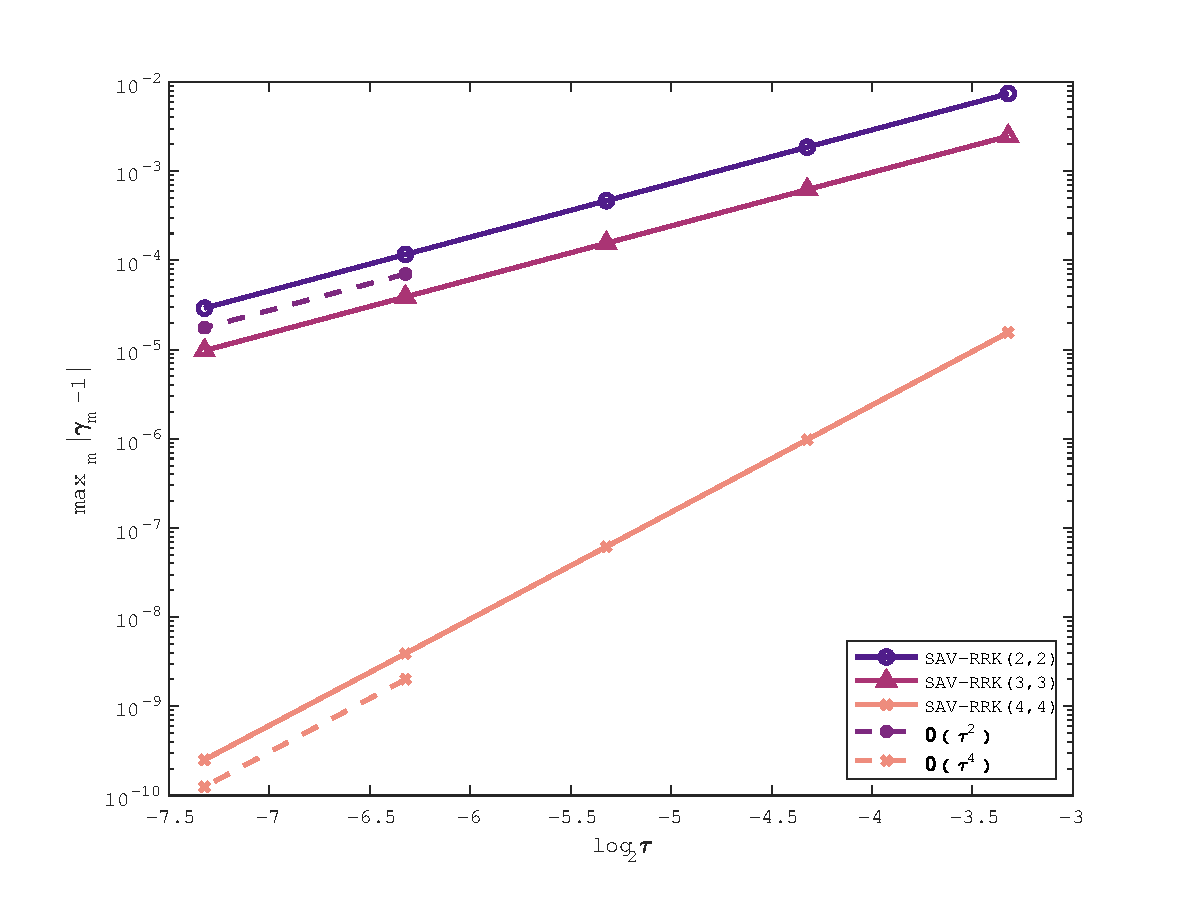
\includegraphics[width=0.5\textwidth]{./figure/exp1_r.eps}
%\centerline{($b$) Spatial accuracy with $\tau = 10^{-3}.$}
}\subfigure[$\max\limits_m\left|S_m(1)\right|$]{ \centering
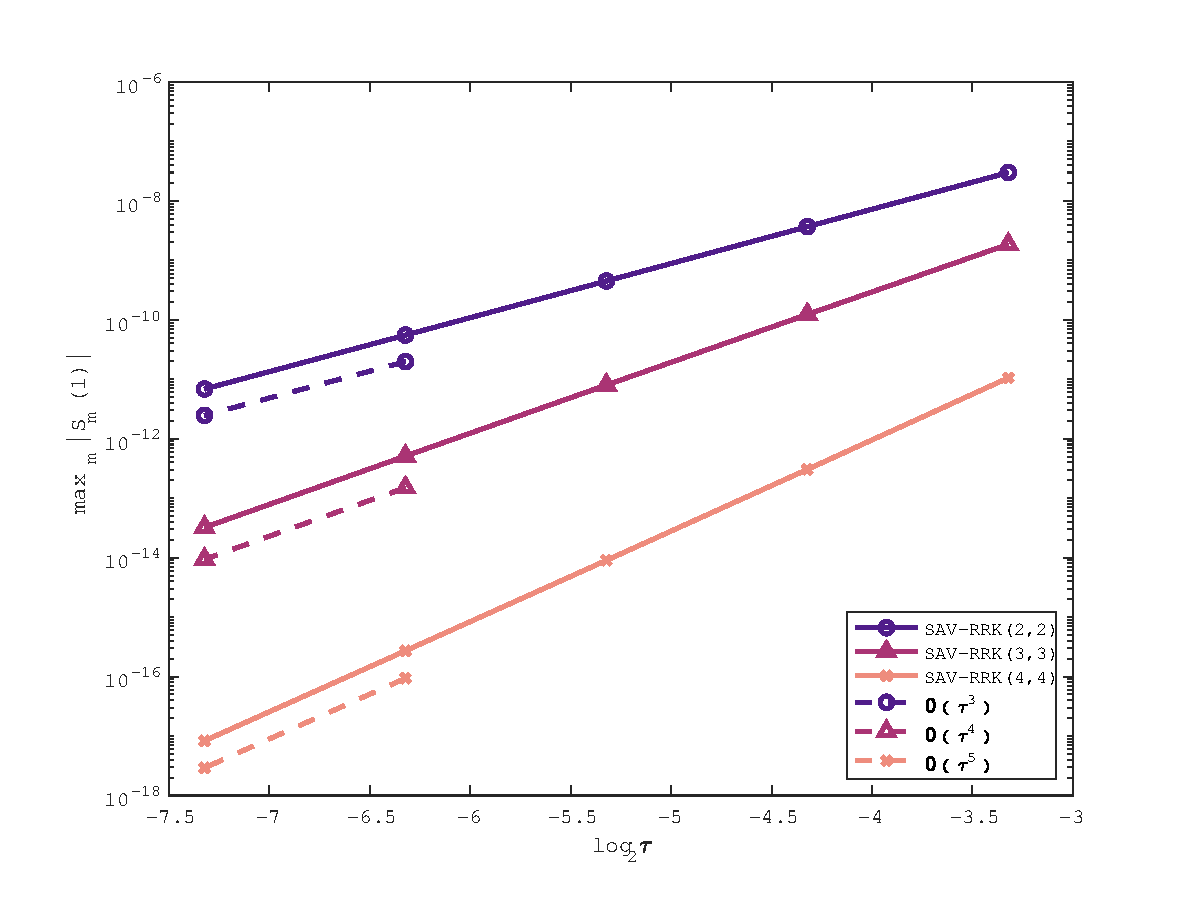
\includegraphics[width=0.5\textwidth]{./figure/exp1_s.eps}
%\centerline{($a$) Temporal accuracy with $N=128.$}
}\caption{$\max\limits_m\left|\gamma_m-1\right|$ and $\max\limits_m\left|S_m(1)\right|$ for some relaxation methods in Example \ref{ex:1}.}
\label{fig:1}
\end{center}
\end{figure}
	

We also run a long time simulation till $T=1000$ and plot the relative energy by the SAV-RRK(4,4) methods with different $\alpha$ in Fig. \ref{fig:4},
which indicates that the proposed schemes can preserve the energy exactly in discrete level and the conservation performance is significantly better
than the SAV method \cite{chengConvergenceEnergyconservingScheme2022} and three-level linearly implicit difference method \cite{wangConservativeLinearizedDifference2015}.
\begin{figure}[H]
\begin{center}
\subfigure[$\alpha=1.3$]{ \centering
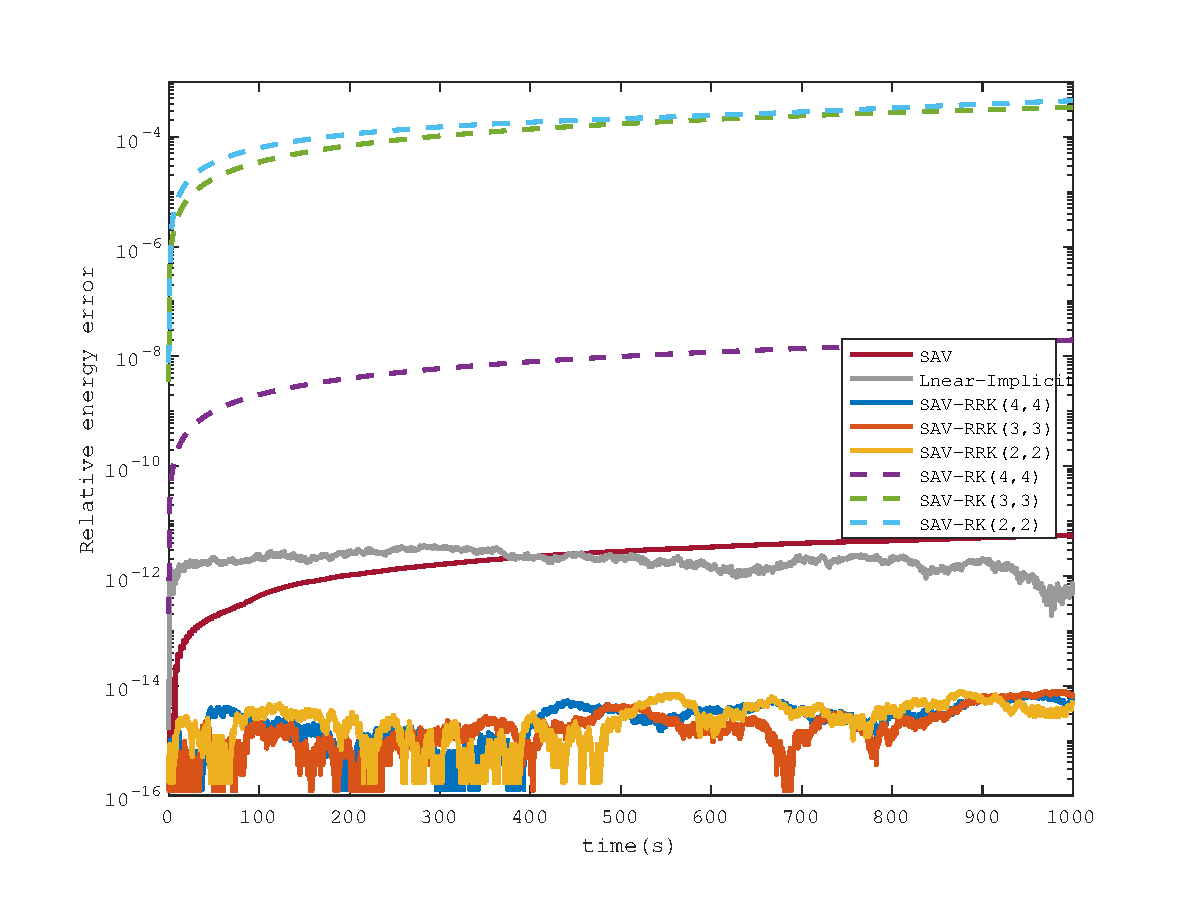
\includegraphics[width=0.5\textwidth]{./figure/exp1_energy3.eps}
%\centerline{($b$) Spatial accuracy with $\tau = 10^{-3}.$}
}\subfigure[$\alpha=1.6$]{ \centering
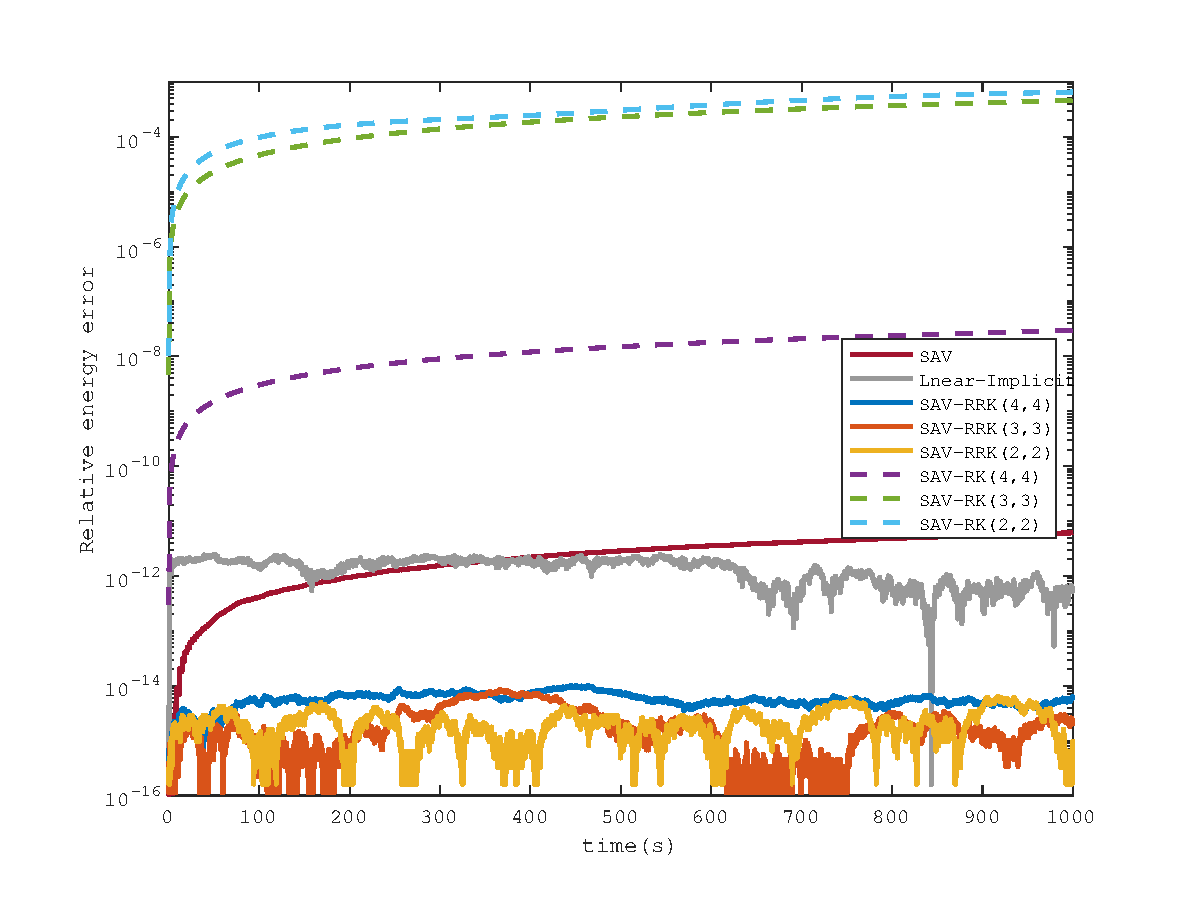
\includegraphics[width=0.5\textwidth]{./figure/exp1_energy6.eps}
%\centerline{($a$) Temporal accuracy with $N=128.$}
}\\
\subfigure[$\alpha=1.9$]{ \centering
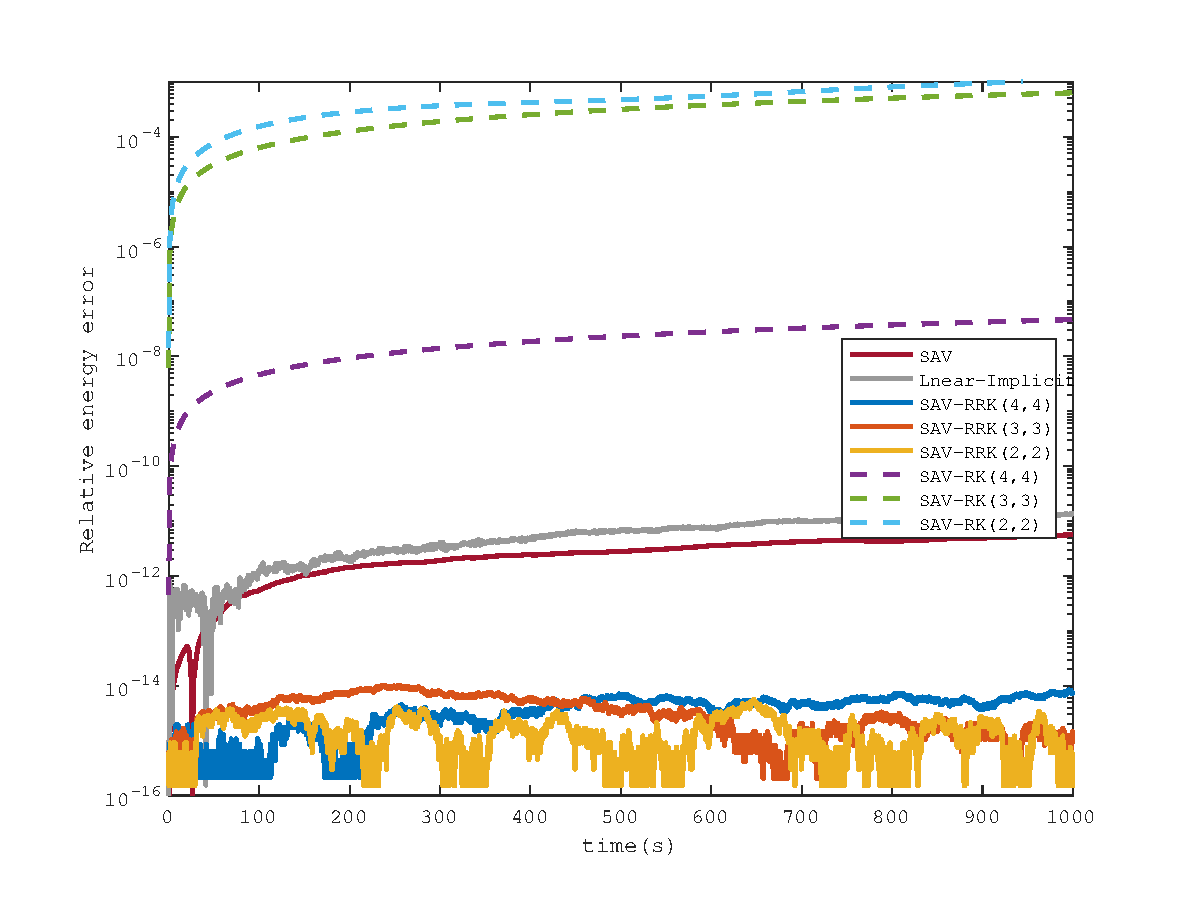
\includegraphics[width=0.5\textwidth]{./figure/exp1_energy9.eps}
%\centerline{($b$) Spatial accuracy with $\tau = 10^{-3}.$}
}\subfigure[$\alpha=2$]{ \centering
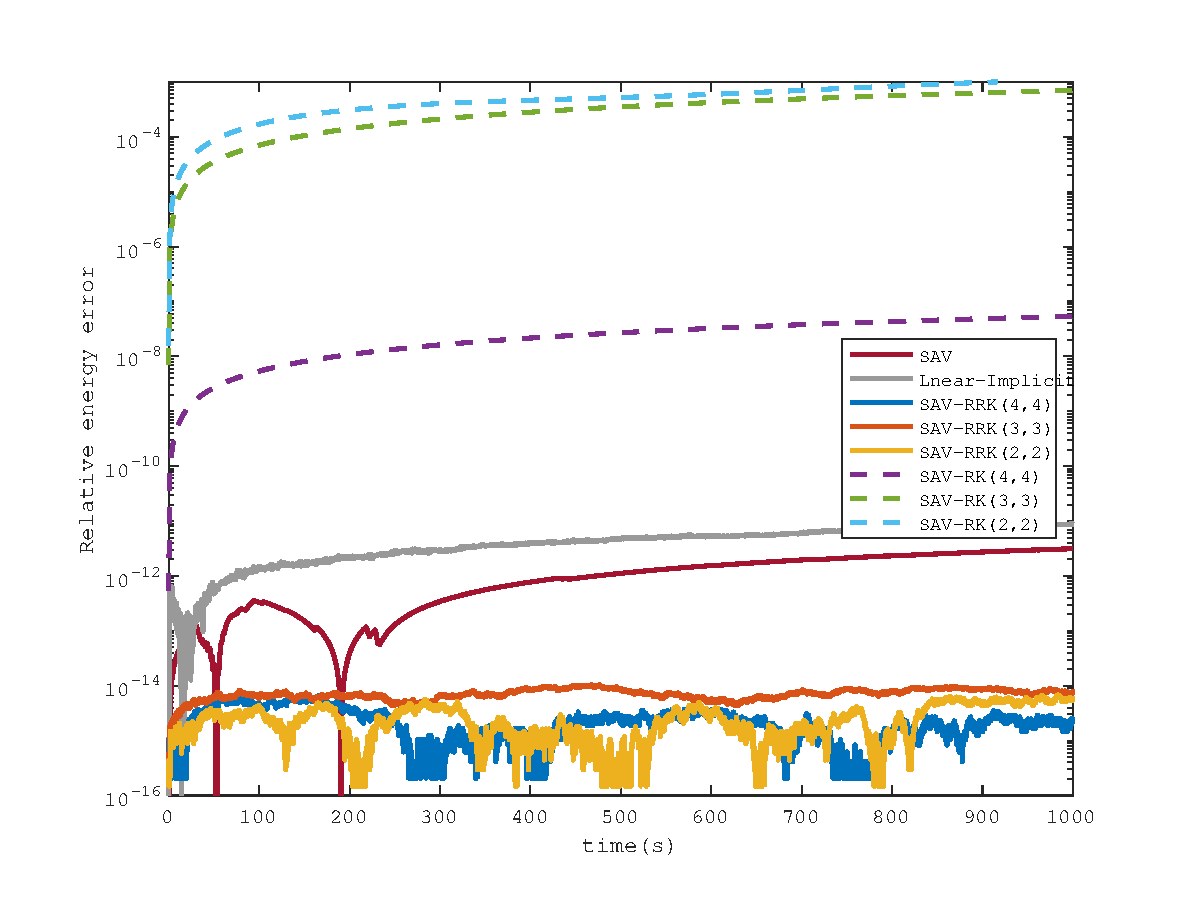
\includegraphics[width=0.5\textwidth]{./figure/exp1_energy2.eps}
%\centerline{($a$) Temporal accuracy with $N=128.$}
}\caption{ Relative errors of energy with $N=32, \tau=0.01$ for different $\alpha$ in Example \ref{ex:1}.}
\label{fig:4}
\end{center}
\end{figure}
	
\begin{example}\label{ex:2}
Now we consider the 2D NFSWEs \eqref{eq_1} with initial values
\begin{equation*}
u(x, y, 0)=\operatorname{sech}\left(x^2+y^2\right), u_t(x, y, 0)=\sin (x+y) \operatorname{sech}\left(-2\left(x^2+y^2\right)\right),(x, y, t) \in \Omega \times[0, T],
\end{equation*}
where $\Omega=[-5,5] \times[-5,5]$.
\end{example}
	
	
In order to reconfirm the applicability of the theoretical results in 2D case,
the same arguments as in Example \ref{ex:1} are considered in the calculation.
That is, $\alpha=1.5$ and $T=1$.  The obtained convergence order in temporal and
the relaxation coefficient $\gamma$ are presented in Table \ref{tab:6-2} and
Fig. \ref{fig:2-1}, respectively. We can observe that the only difference from the 1D case is that the SAV-RRK(IDT) methods do not achieve a higher-than-expected
order in the 2D case.
	
\begin{table}[H]\footnotesize
\centering
\caption{Numerical errors and convergence order in time for Example \ref{ex:2} when $N=4, T = 1$.}
\begin{tabular}{lllllrlrlrlrlrl}
\toprule
\multicolumn{2}{l}{\multirow{2}[3]{*}{\textbf{RK(Stage,Order)}}} & \multicolumn{2}{l}{\multirow{2}[3]{*}{$\bm{\tau}$}} & \multicolumn{3}{c}{\textbf{SAV-RK}} &       & \multicolumn{3}{c}{\textbf{SAV-RRK}} &       & \multicolumn{3}{c}{\textbf{SAV-RRK(IDT)}} \\
\cmidrule{5-7}\cmidrule{9-11}\cmidrule{13-15}    \multicolumn{2}{l}{} & \multicolumn{2}{l}{} & \textbf{Error($\tau$)} &       & \textbf{order} &       & \textbf{Error($\tau$)} &       & \textbf{order} &       & \textbf{Error($\tau$)} &       & \textbf{order} \\
\hline
\multicolumn{2}{l}{\multirow{5}[0]{*}{\textbf{RK(2,2)}}} & \multicolumn{2}{l}{0.1} & 3.0217E-03 &       & -     &       & 3.0102E-03 &       & -     &       & 1.5692E-02 &       & - \\
\multicolumn{2}{l}{} & \multicolumn{2}{l}{0.05} & 7.4615E-04 &       & 2.0178  &       & 7.4702E-04 &       & 2.0106  &       & 9.6213E-03 &       & 0.7057  \\
\multicolumn{2}{l}{} & \multicolumn{2}{l}{0.025} & 1.8513E-04 &       & 2.0109  &       & 1.8587E-04 &       & 2.0069  &       & 5.2472E-03 &       & 0.8747  \\
\multicolumn{2}{l}{} & \multicolumn{2}{l}{0.0125} & 4.6090E-05 &       & 2.0060  &       & 4.6341E-05 &       & 2.0039  &       & 2.7312E-03 &       & 0.9420  \\
\multicolumn{2}{l}{} & \multicolumn{2}{l}{0.00625} & 1.1497E-05 &       & 2.0032  &       & 1.1569E-05 &       & 2.0021  &       & 1.3923E-03 &       & 0.9721  \\
\multicolumn{2}{l}{\multirow{5}[0]{*}{\textbf{RK(3,3)}}} & \multicolumn{2}{l}{0.1} & 1.2581E-04 &       & -     &       & 3.9379E-05 &       & -     &       & 3.2535E-03 &       & - \\
\multicolumn{2}{l}{} & \multicolumn{2}{l}{0.05} & 1.6180E-05 &       & 2.9589  &       & 5.5726E-06 &       & 2.8210  &       & 7.9304E-04 &       & 2.0365  \\
\multicolumn{2}{l}{} & \multicolumn{2}{l}{0.025} & 2.0532E-06 &       & 2.9783  &       & 7.4443E-07 &       & 2.9041  &       & 1.9546E-04 &       & 2.0205  \\
\multicolumn{2}{l}{} & \multicolumn{2}{l}{0.0125} & 2.5863E-07 &       & 2.9889  &       & 9.6210E-08 &       & 2.9519  &       & 4.8500E-05 &       & 2.0108  \\
\multicolumn{2}{l}{} & \multicolumn{2}{l}{0.00625} & 3.2454E-08 &       & 2.9944  &       & 1.2228E-08 &       & 2.9760  &       & 1.2078E-05 &       & 2.0056  \\
\multicolumn{2}{l}{\multirow{5}[1]{*}{\textbf{RK(4,4)}}} & \multicolumn{2}{l}{0.1} & 7.9185E-06 &       & -     &       & 8.0508E-06 &       & -     &       & 3.4013E-05 &       & - \\
\multicolumn{2}{l}{} & \multicolumn{2}{l}{0.05} & 4.9103E-07 &       & 4.0113  &       & 4.9644E-07 &       & 4.0194  &       & 3.3898E-06 &       & 3.3268  \\
\multicolumn{2}{l}{} & \multicolumn{2}{l}{0.025} & 3.0531E-08 &       & 4.0075  &       & 3.0805E-08 &       & 4.0104  &       & 3.6901E-07 &       & 3.1995  \\
\multicolumn{2}{l}{} & \multicolumn{2}{l}{0.0125} & 1.9026E-09 &       & 4.0042  &       & 1.9182E-09 &       & 4.0054  &       & 4.2681E-08 &       & 3.1120  \\
\multicolumn{2}{l}{} & \multicolumn{2}{l}{0.00625} & 1.1873E-10 &       & 4.0022  &       & 1.1966E-10 &       & 4.0027  &       & 5.1191E-09 &       & 3.0596  \\
\bottomrule
\end{tabular}%
\label{tab:6-2}%
\end{table}%
	
\begin{figure}[H]
\begin{center}
\subfigure[$\max _m\left|\gamma_m-1\right|$]{ \centering
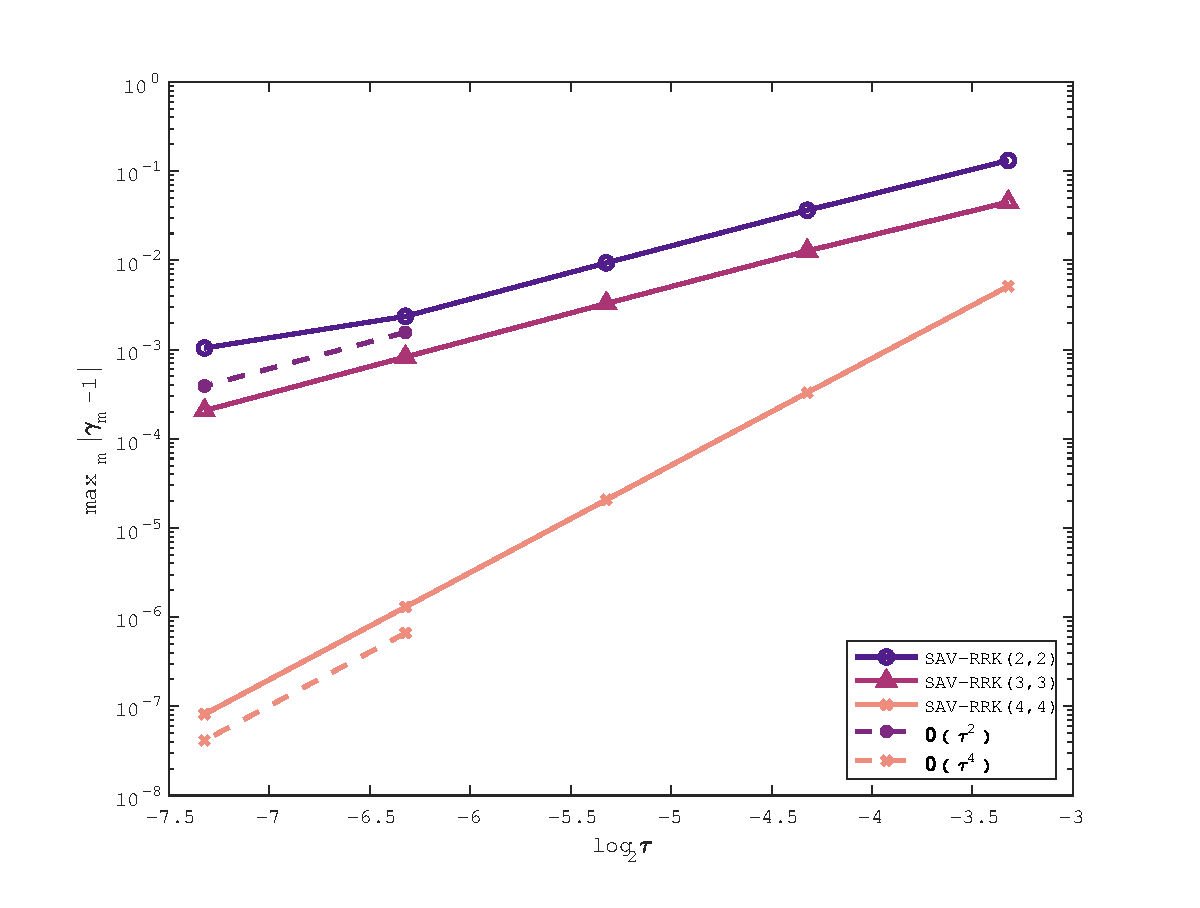
\includegraphics[width=0.5\textwidth]{./figure/exp2_r.eps}
%\centerline{($b$) Spatial accuracy with $\tau = 10^{-3}.$}
}\subfigure[$\max_m\left|S_m(1)\right|$]{ \centering
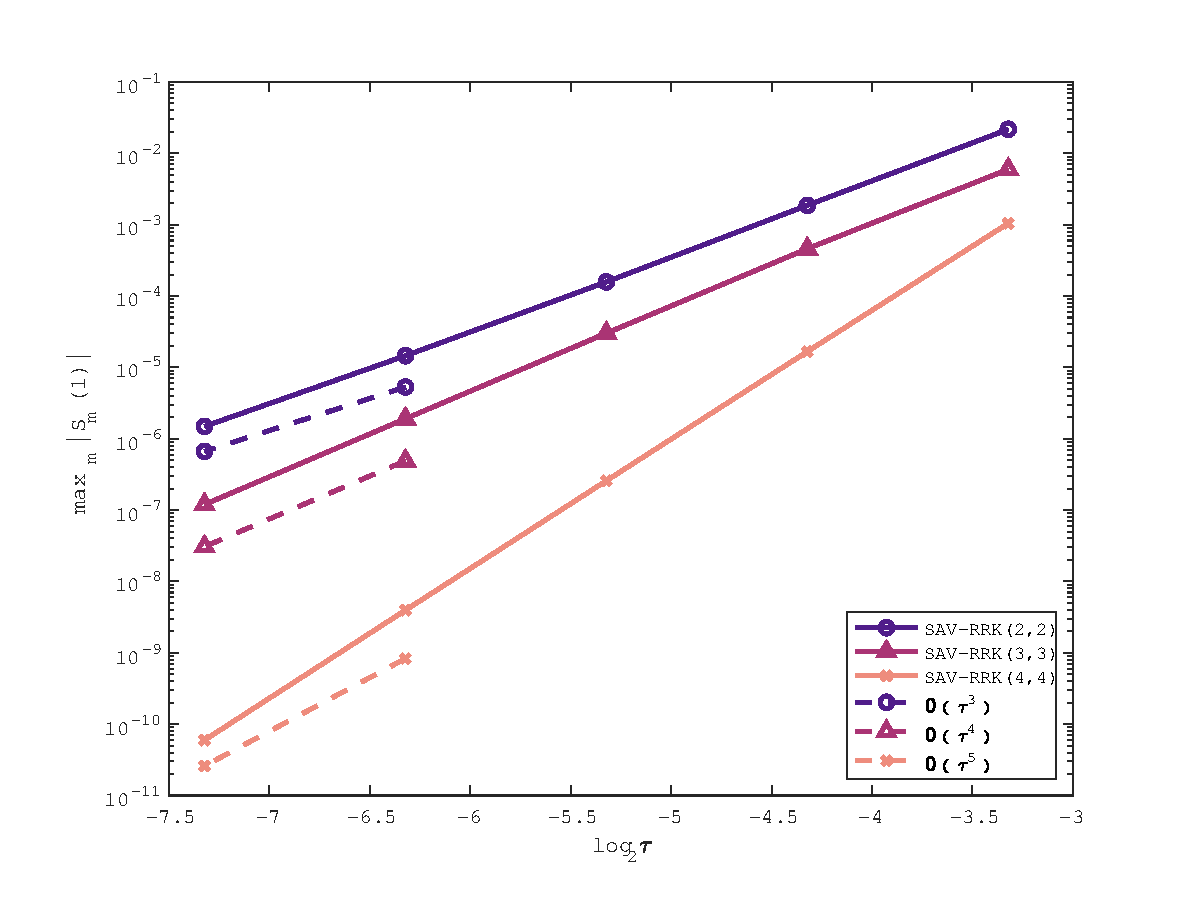
\includegraphics[width=0.5\textwidth]{./figure/exp2_s.eps}
%\centerline{($a$) Temporal accuracy with $N=128.$}
}\caption{$\max _m\left|\gamma_m-1\right|$ and $\max_m\left|S_m(1)\right|$ for some relaxation (RT) methods in Example \ref{ex:2}.}
\label{fig:2-1}
\end{center}
\end{figure}
	

To demonstrate the effectiveness of the proposed methods in preserving
energy, we perform long time simulations until $T=100$ and plot the
relative energy errors using the SAV-RRK(4,4) methods with different
$\alpha$ in Fig. \ref{fig:2-4}. The results reveal that the proposed methods can preserve energy exactly at the discrete level, and the
conservation performance is significantly better than that of the SAV
method \cite{chengConvergenceEnergyconservingScheme2022}.
\begin{figure}[H]
\begin{center}
\subfigure[$\alpha=1.3$]{ \centering
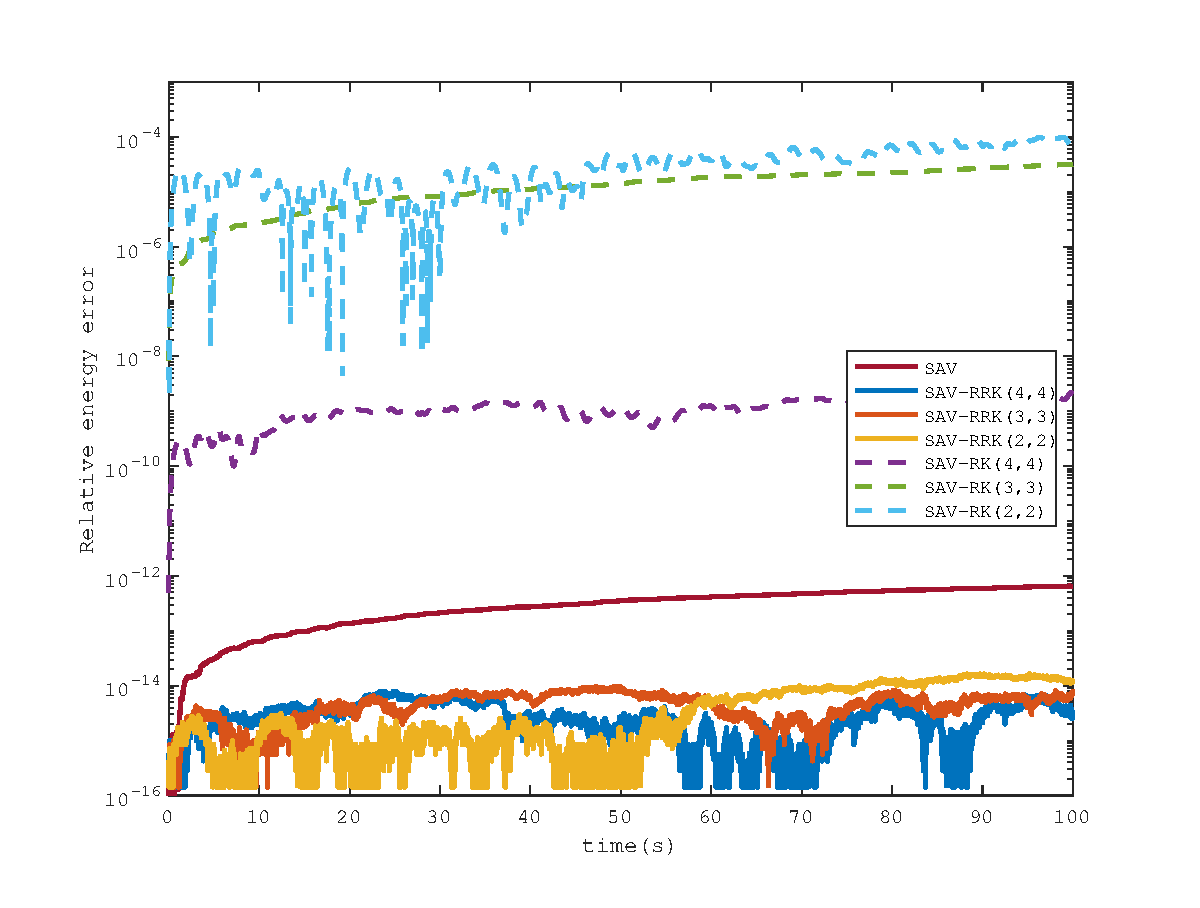
\includegraphics[width=0.5\textwidth]{./figure/exp2_energy3.eps}
%\centerline{($b$) Spatial accuracy with $\tau = 10^{-3}.$}
}\subfigure[$\alpha=1.6$]{ \centering
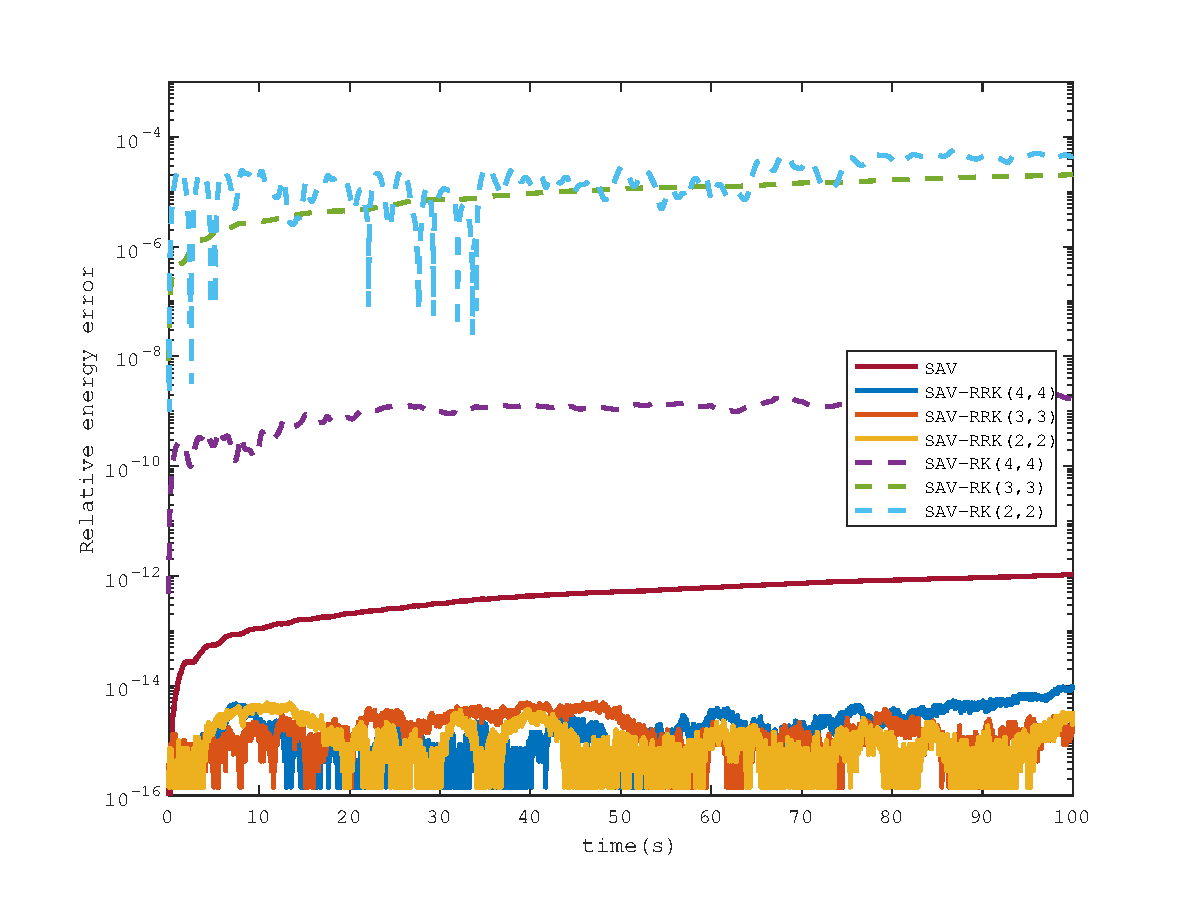
\includegraphics[width=0.5\textwidth]{./figure/exp2_energy6.eps}
%\centerline{($a$) Temporal accuracy with $N=128.$}
}\\
\subfigure[$\alpha=1.9$]{ \centering
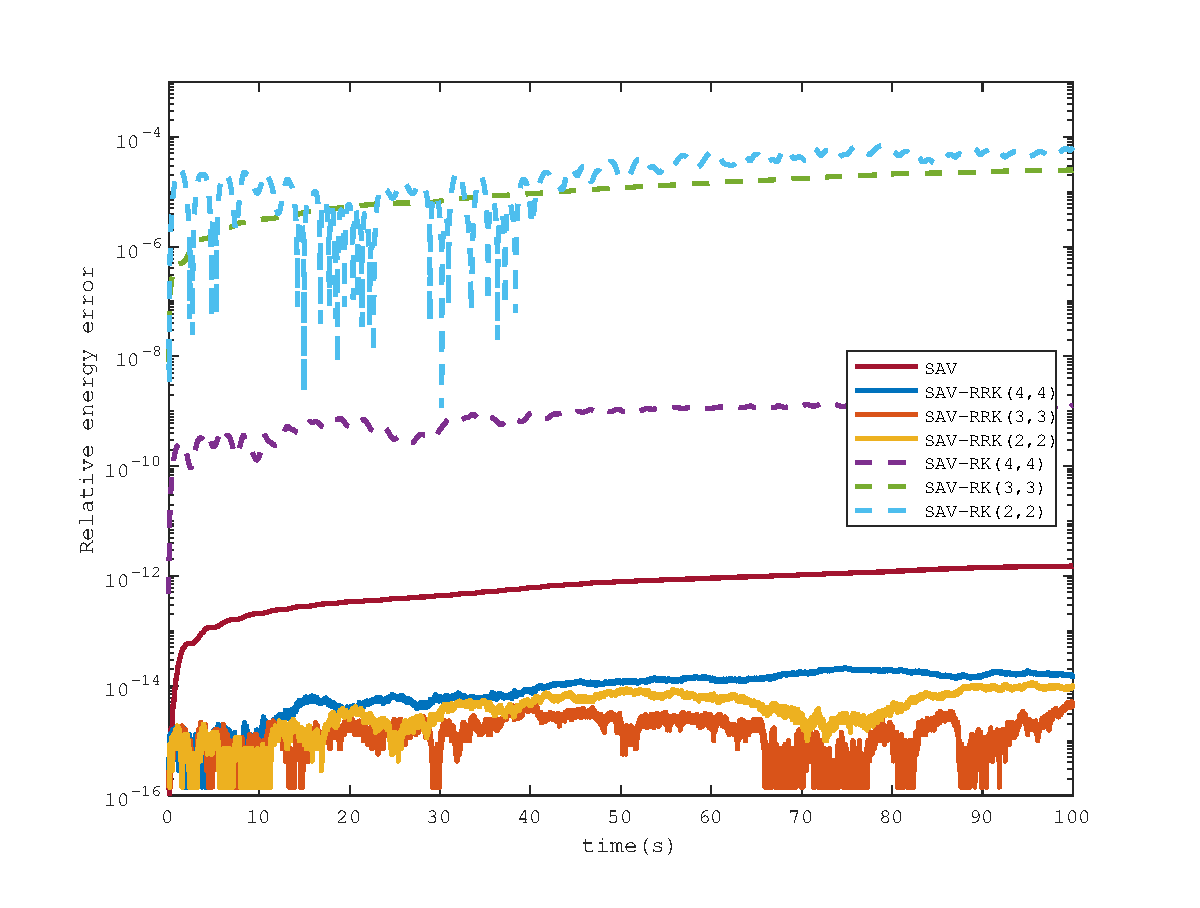
\includegraphics[width=0.5\textwidth]{./figure/exp2_energy9.eps}
%\centerline{($b$) Spatial accuracy with $\tau = 10^{-3}.$}
}\subfigure[$\alpha=2$]{ \centering
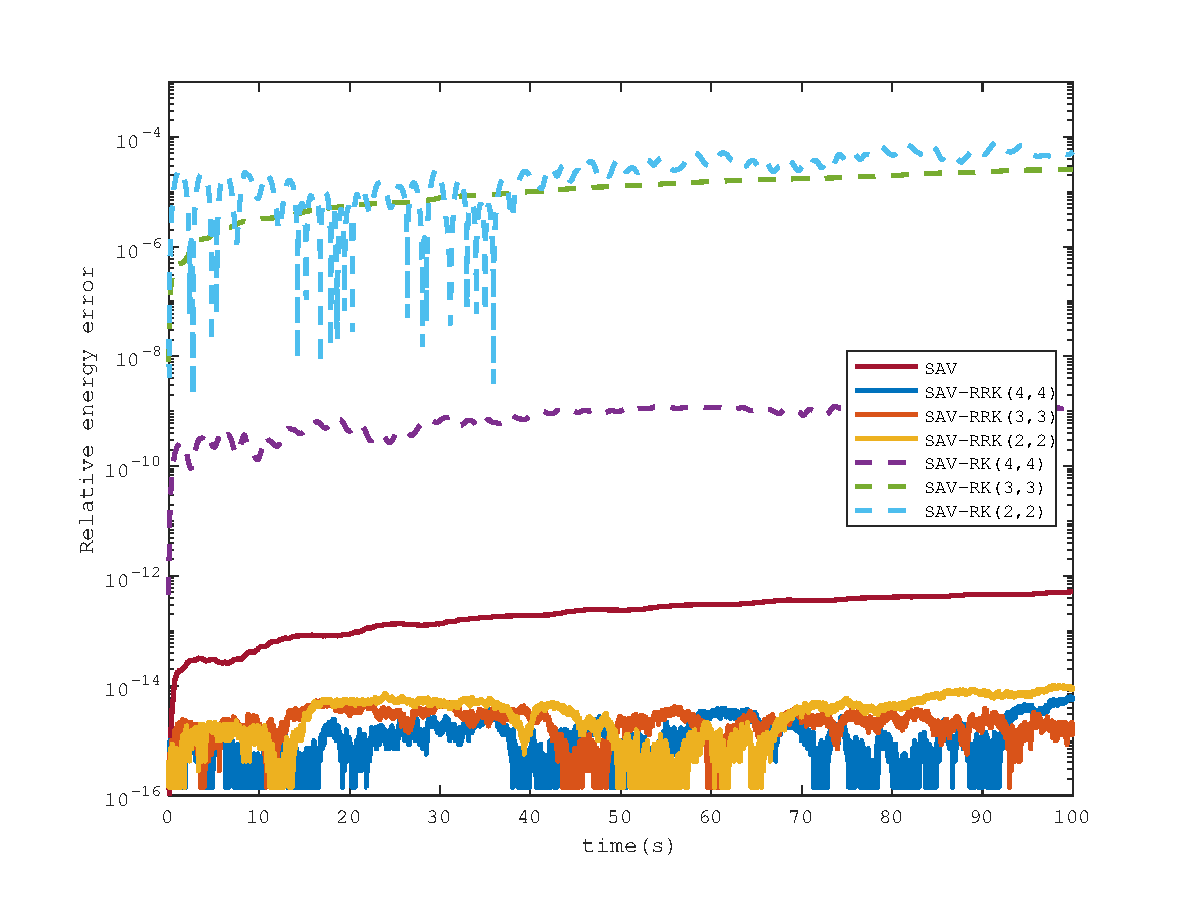
\includegraphics[width=0.5\textwidth]{./figure/exp2_energy2.eps}
%\centerline{($a$) Temporal accuracy with $N=128.$}
}\caption{ Relative errors of energy with $N=4, \tau=0.01$ for different $\alpha$ in Example \ref{ex:2}.}
\label{fig:2-4}
\end{center}
\end{figure}
	
\begin{example}\label{ex:3}
\cite{wangUnconditionalEnergyDissipation2021} Next, we consider the 2D nonlinear fractional wave equation
\begin{equation}
\begin{cases}
& u_{t t}+(-\Delta)^{\frac{\alpha}{2}} u+F^{\prime}(u)=0,(x, y, t) \in \Omega \times(0, T],\\
& u(x, y, 0)=\frac{1}{2} \arctan \left(\exp \left(-\sqrt{x^2+y^2}\right)\right), u_t(x, y, 0)=0,
\end{cases}
\end{equation}
where $\Omega=(-10,10) \times(-10,10)$.
\end{example}

Taking the potential energy $F(u)=u^2\left(\frac{1}{4} u^2-\frac{1}{2}\right)$. The convergence order
in time for $\alpha=1.5$ at $T=1$ is shown in Table \ref{tab:6-3}.
Also, the evolution of discrete energy for a long-time simulation ($T=100$) is depicted in Fig. \ref{fig:3-4}.
These data is calculated by applying the SAV-RRK(4,4) method. The results indicate that the proposed methods
is also valid for the nonlinear fractional wave equations.
\begin{table}[H]\footnotesize
\centering
\caption{Numerical errors and convergence order in time for Example \ref{ex:3} when $N=4, T = 1$.}
\begin{tabular}{lllllrlrlrlrlrl}
\toprule
\multicolumn{2}{l}{\multirow{2}[3]{*}{\textbf{RK(Stage,Order)}}} & \multicolumn{2}{l}{\multirow{2}[3]{*}{$\bm{\tau}$}} & \multicolumn{3}{c}{\textbf{SAV-RK}} &       & \multicolumn{3}{c}{\textbf{SAV-RRK(RT)}} &       & \multicolumn{3}{c}{\textbf{SAV-RRK(IDT)}} \\
\cmidrule{5-7}\cmidrule{9-11}\cmidrule{13-15}    \multicolumn{2}{l}{} & \multicolumn{2}{l}{} & \textbf{Error($\tau$)} &       & \textbf{order} &       & \textbf{Error($\tau$)} &       & \textbf{order} &       & \textbf{Error($\tau$)} &       & \textbf{order} \\
\hline
\multicolumn{2}{l}{\multirow{5}[0]{*}{\textbf{RK(2,2)}}} & \multicolumn{2}{l}{0.1} & 1.3395E-03 &       & -     &       & 3.3870E-03 &       & -     &       & 2.1470E-02 &       & - \\
\multicolumn{2}{l}{} & \multicolumn{2}{l}{0.05} & 3.4360E-04 &       & 1.9628  &       & 8.1480E-04 &       & 2.0555  &       & 1.0960E-02 &       & 0.9701  \\
\multicolumn{2}{l}{} & \multicolumn{2}{l}{0.025} & 8.6945E-05 &       & 1.9826  &       & 1.9951E-04 &       & 2.0300  &       & 5.5113E-03 &       & 0.9918  \\
\multicolumn{2}{l}{} & \multicolumn{2}{l}{0.0125} & 2.1865E-05 &       & 1.9915  &       & 4.9347E-05 &       & 2.0154  &       & 2.7600E-03 &       & 0.9977  \\
\multicolumn{2}{l}{} & \multicolumn{2}{l}{0.00625} & 5.4823E-06 &       & 1.9958  &       & 1.2270E-05 &       & 2.0078  &       & 1.3807E-03 &       & 0.9993  \\
\multicolumn{2}{l}{\multirow{5}[0]{*}{\textbf{RK(3,3)}}} & \multicolumn{2}{l}{0.1} & 3.5168E-05 &       & -     &       & 4.3927E-05 &       & -     &       & 3.8213E-04 &       & - \\
\multicolumn{2}{l}{} & \multicolumn{2}{l}{0.05} & 4.3533E-06 &       & 3.0141  &       & 5.4825E-06 &       & 3.0022  &       & 8.0473E-05 &       & 2.2475  \\
\multicolumn{2}{l}{} & \multicolumn{2}{l}{0.025} & 5.3902E-07 &       & 3.0137  &       & 6.8378E-07 &       & 3.0032  &       & 1.8560E-05 &       & 2.1163  \\
\multicolumn{2}{l}{} & \multicolumn{2}{l}{0.0125} & 6.7058E-08 &       & 3.0068  &       & 8.5344E-08 &       & 3.0022  &       & 4.4475E-06 &       & 2.0611  \\
\multicolumn{2}{l}{} & \multicolumn{2}{l}{0.00625} & 8.3615E-09 &       & 3.0036  &       & 1.0659E-08 &       & 3.0012  &       & 1.0883E-06 &       & 2.0309  \\
\multicolumn{2}{l}{\multirow{5}[1]{*}{\textbf{RK(4,4)}}} & \multicolumn{2}{l}{0.1} & 5.3561E-07 &       & -     &       & 3.2716E-06 &       & -     &       & 3.7745E-05 &       & - \\
\multicolumn{2}{l}{} & \multicolumn{2}{l}{0.05} & 3.6438E-08 &       & 3.8777  &       & 2.0654E-07 &       & 3.9855  &       & 4.8050E-06 &       & 2.9737  \\
\multicolumn{2}{l}{} & \multicolumn{2}{l}{0.025} & 2.3735E-09 &       & 3.9403  &       & 1.2898E-08 &       & 4.0012  &       & 6.0237E-07 &       & 2.9958  \\
\multicolumn{2}{l}{} & \multicolumn{2}{l}{0.0125} & 1.5146E-10 &       & 3.9700  &       & 8.0476E-10 &       & 4.0024  &       & 7.5303E-08 &       & 2.9999  \\
\multicolumn{2}{l}{} & \multicolumn{2}{l}{0.00625} & 9.5636E-12 &       & 3.9853  &       & 5.0241E-11 &       & 4.0016  &       & 9.4105E-09 &       & 3.0004  \\
\bottomrule
\end{tabular}%
\label{tab:6-3}%
\end{table}%
\vspace{-10mm}

\begin{figure}[H]
\begin{center}
\subfigure[$\alpha=1.3$]{ \centering
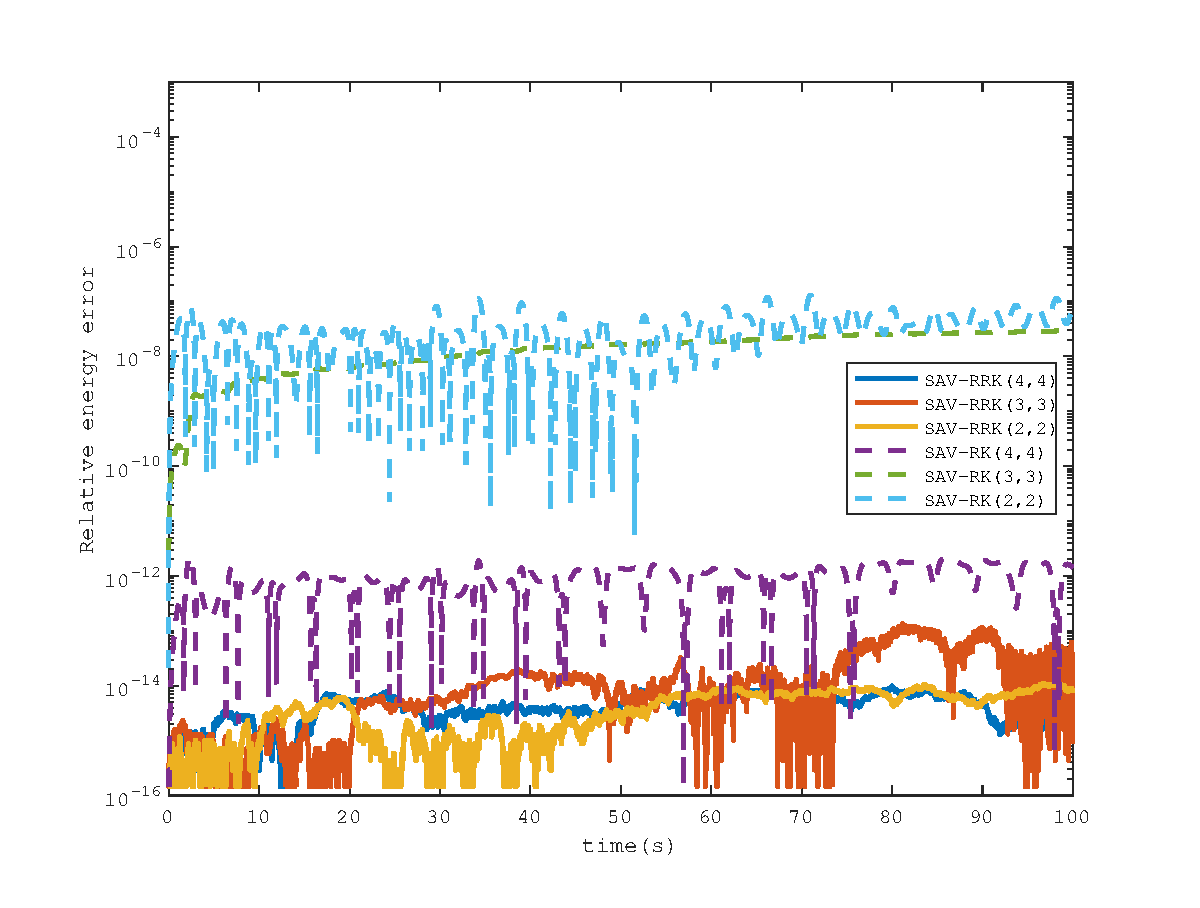
\includegraphics[width=0.5\textwidth]{./figure/exp3_energy3.eps}
%\centerline{($b$) Spatial accuracy with $\tau = 10^{-3}.$}
}\subfigure[$\alpha=1.6$]{ \centering
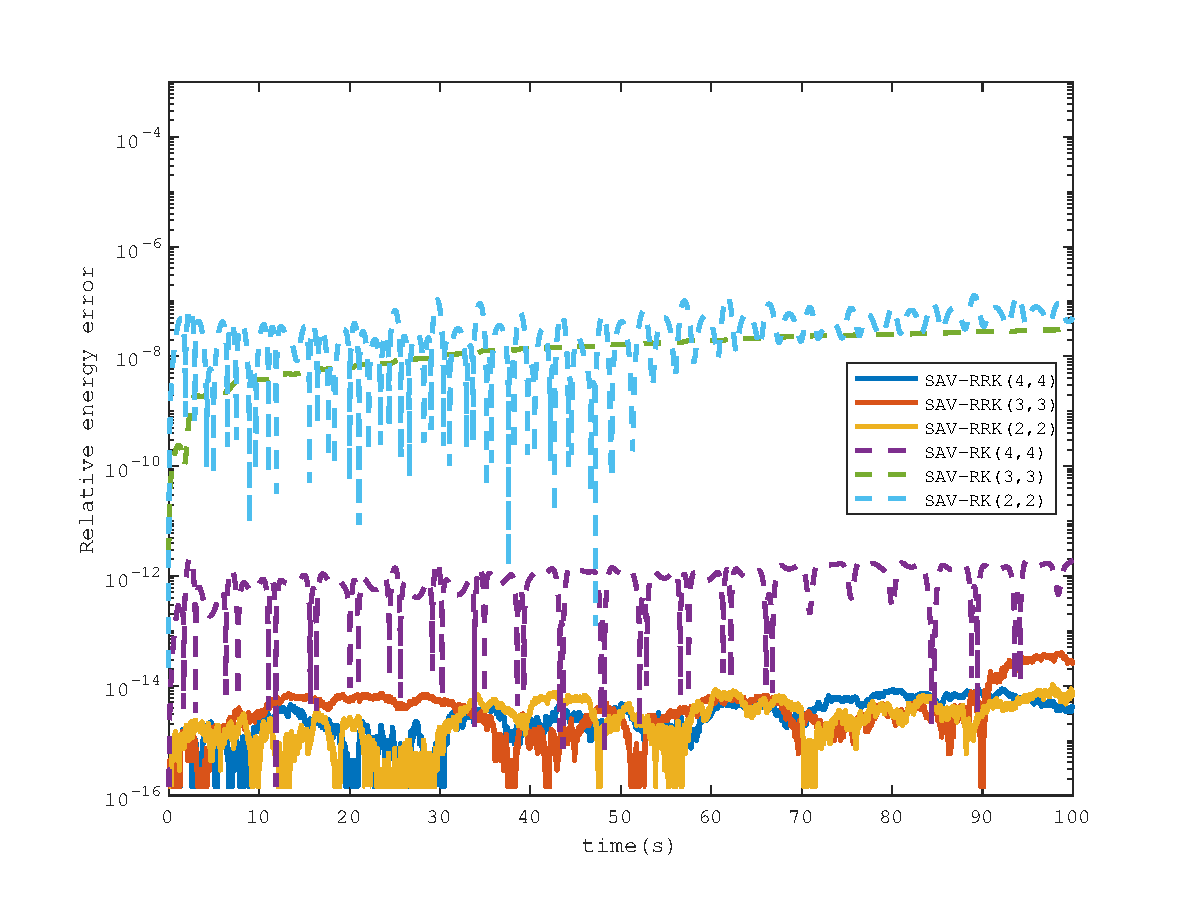
\includegraphics[width=0.5\textwidth]{./figure/exp3_energy6.eps}
%\centerline{($a$) Temporal accuracy with $N=128.$}
}\\
\subfigure[$\alpha=1.9$]{ \centering
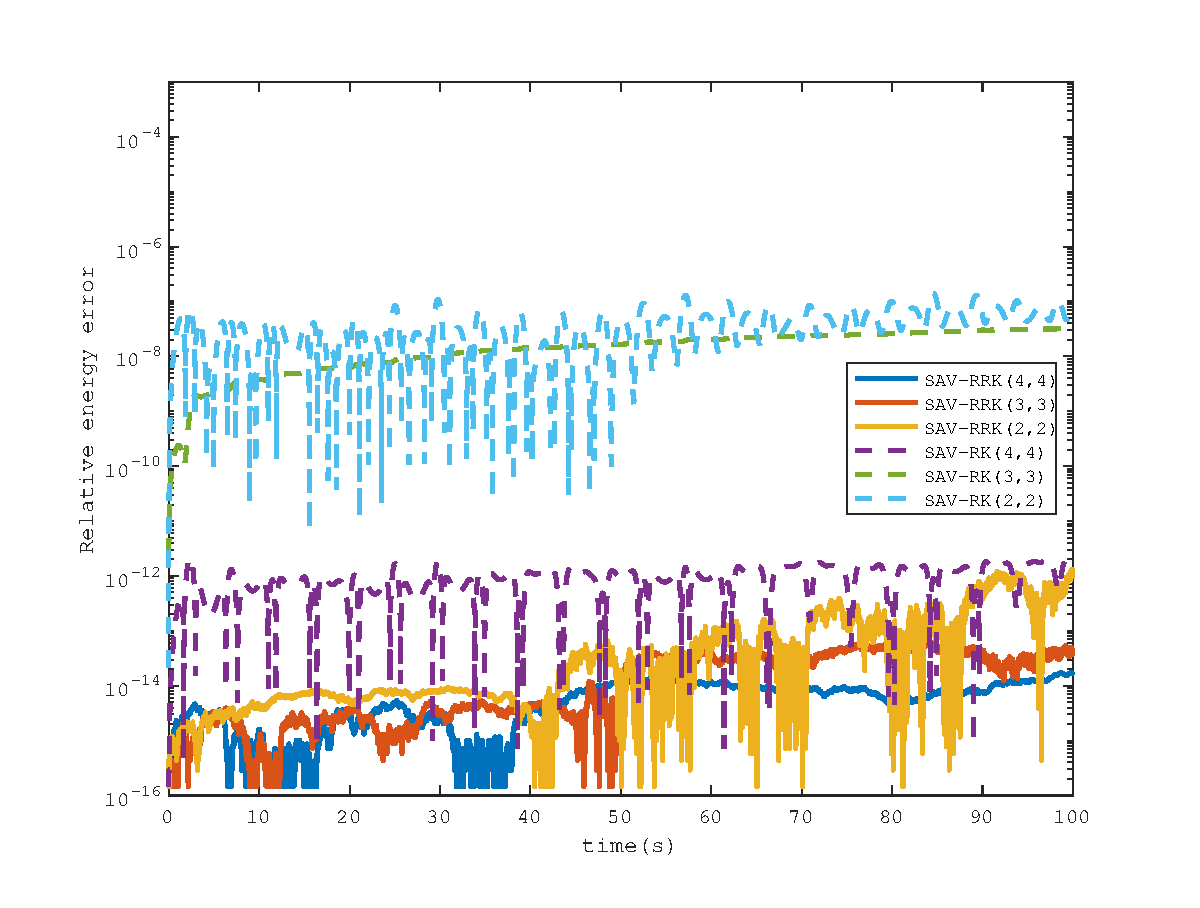
\includegraphics[width=0.5\textwidth]{./figure/exp3_energy9.eps}
%\centerline{($b$) Spatial accuracy with $\tau = 10^{-3}.$}
}\subfigure[$\alpha=2$]{ \centering
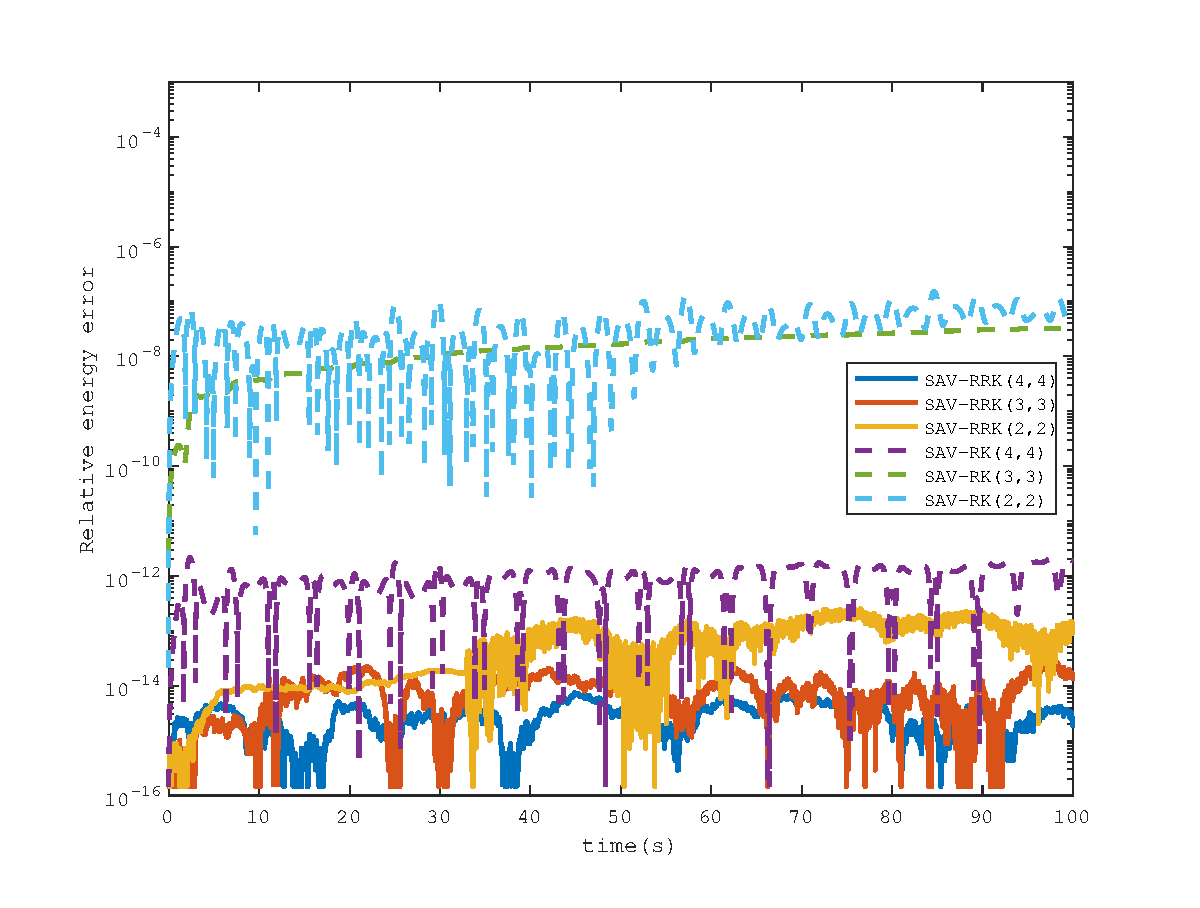
\includegraphics[width=0.5\textwidth]{./figure/exp3_energy2.eps}
%\centerline{($a$) Temporal accuracy with $N=128.$}
}\caption{ Relative errors of energy with $N=4, \tau=0.01$ for different $\alpha$ in Example \ref{ex:3}.}
\label{fig:3-4}
\end{center}
\end{figure}

\begin{example}\label{ex:4}
\cite{fuStructurepreservingAlgorithmsTwodimensional2020}
Finally, we consider the 2D fractional Klein-Gordon-Schr{\"o}dinger equation
\begin{equation}
\begin{cases}
\mathrm{i} \partial_t u-\frac{1}{2}(-\Delta)^{\frac{\alpha}{2}} u+u \phi=0,(x, y, t) \in \Omega \times(0, T],\\
\partial_{t t} \phi+(-\Delta)^{\frac{\beta}{2}} \phi+\phi-|u|^2=0, (x, y, t) \in \Omega \times(0, T],
\end{cases}
\end{equation}
with the initial conditions
\begin{equation}
u(x, y, 0)=(1+\mathrm{i}) \exp \left(-|\boldsymbol{x}|^2\right),~~\phi(x, y, 0)=\operatorname{sech}\left(|\boldsymbol{x}|^2\right),~~ \partial_t \phi(x, y, 0)=\sin (x+y) \operatorname{sech}\left(-2|\boldsymbol{x}|^2\right),
\end{equation}
where $\Omega=[-10,10] \times[-10,10]$.
\end{example}

Similar to the previous examples, some numerical errors and convergence order in time are listed in Table \ref{tab:6-4}
for $\alpha=\beta=1.5$.

\begin{table}[H]\footnotesize
\centering
\caption{Numerical errors and convergence order in time for Example \ref{ex:4} when $N=4, T = 1$.}
\begin{tabular}{lllllrlrlrlrlrl}
\toprule
\multicolumn{2}{l}{\multirow{2}[3]{*}{\textbf{RK(Stage,Order)}}} & \multicolumn{2}{l}{\multirow{2}[3]{*}{$\bm{\tau}$}} & \multicolumn{3}{c}{\textbf{SAV-RK}} &       & \multicolumn{3}{c}{\textbf{SAV-RRK(RT)}} &       & \multicolumn{3}{c}{\textbf{SAV-RRK(IDT)}} \\
\cmidrule{5-7}\cmidrule{9-11}\cmidrule{13-15}    \multicolumn{2}{l}{} & \multicolumn{2}{l}{} & \textbf{Error($\tau$)} &       & \textbf{order} &       & \textbf{Error($\tau$)} &       & \textbf{order} &       & \textbf{Error($\tau$)} &       & \textbf{order} \\
\hline
\multicolumn{2}{l}{\multirow{5}[0]{*}{\textbf{RK(2,2)}}} & \multicolumn{2}{l}{0.1} & 1.1875E-03 &       & -     &       & 1.8837E-03 &       & -     &       & 9.5325E-03 &       & - \\
\multicolumn{2}{l}{} & \multicolumn{2}{l}{0.05} & 2.7648E-04 &       & 2.1026  &       & 5.0394E-04 &       & 1.9023  &       & 6.7134E-03 &       & 0.5058  \\
\multicolumn{2}{l}{} & \multicolumn{2}{l}{0.025} & 6.6514E-05 &       & 2.0555  &       & 1.3036E-04 &       & 1.9508  &       & 3.8805E-03 &       & 0.7908  \\
\multicolumn{2}{l}{} & \multicolumn{2}{l}{0.0125} & 1.6300E-05 &       & 2.0288  &       & 3.3151E-05 &       & 1.9754  &       & 2.0757E-03 &       & 0.9026  \\
\multicolumn{2}{l}{} & \multicolumn{2}{l}{0.00625} & 4.0339E-06 &       & 2.0146  &       & 8.3587E-06 &       & 1.9877  &       & 1.0723E-03 &       & 0.9529  \\
\multicolumn{2}{l}{\multirow{5}[0]{*}{\textbf{RK(3,3)}}} & \multicolumn{2}{l}{0.1} & 8.7748E-05 &       & -     &       & 1.9567E-04 &       & -     &       & 3.1789E-03 &       & - \\
\multicolumn{2}{l}{} & \multicolumn{2}{l}{0.05} & 1.1471E-05 &       & 2.9354  &       & 2.4630E-05 &       & 2.9900  &       & 8.2646E-04 &       & 1.9435  \\
\multicolumn{2}{l}{} & \multicolumn{2}{l}{0.025} & 1.4684E-06 &       & 2.9657  &       & 3.0916E-06 &       & 2.9940  &       & 2.1079E-04 &       & 1.9712  \\
\multicolumn{2}{l}{} & \multicolumn{2}{l}{0.0125} & 1.8580E-07 &       & 2.9824  &       & 3.8731E-07 &       & 2.9968  &       & 5.3231E-05 &       & 1.9854  \\
\multicolumn{2}{l}{} & \multicolumn{2}{l}{0.00625} & 2.3370E-08 &       & 2.9911  &       & 4.8471E-08 &       & 2.9983  &       & 1.3375E-05 &       & 1.9927  \\
\multicolumn{2}{l}{\multirow{5}[1]{*}{\textbf{RK(4,4)}}} & \multicolumn{2}{l}{0.1} & 3.0741E-06 &       & -     &       & 4.0627E-06 &       & -     &       & 1.0278E-04 &       & - \\
\multicolumn{2}{l}{} & \multicolumn{2}{l}{0.05} & 1.9959E-07 &       & 3.9450  &       & 2.6020E-07 &       & 3.9647  &       & 1.3195E-05 &       & 2.9615  \\
\multicolumn{2}{l}{} & \multicolumn{2}{l}{0.025} & 1.2698E-08 &       & 3.9744  &       & 1.6461E-08 &       & 3.9825  &       & 1.6711E-06 &       & 2.9811  \\
\multicolumn{2}{l}{} & \multicolumn{2}{l}{0.0125} & 8.0044E-10 &       & 3.9876  &       & 1.0350E-09 &       & 3.9913  &       & 2.1024E-07 &       & 2.9906  \\
\multicolumn{2}{l}{} & \multicolumn{2}{l}{0.00625} & 5.0238E-11 &       & 3.9939  &       & 6.4882E-11 &       & 3.9957  &       & 2.6365E-08 &       & 2.9953  \\
\bottomrule
\end{tabular}%
\label{tab:6-4}%
\end{table}%
		
Furthermore, the relative energy with different $\alpha$ and $\beta$ in a long-time simulation up to $T=100$ is described in Fig. \ref{fig:3-5}.
% The phenomenon shown by the image shows that the proposed schemes can accurately preserve energy in the discrete level for the fractional Klein-Gordon-Schr{\"o}dinger equation.
The phenomenon depicted demonstrates that the proposed methods accurately preserve energy at the discrete level for the fractional Klein-Gordon-Schr{\"o}dinger equation.
\begin{figure}[H]
\begin{center}
\subfigure[$\alpha,\beta=1.3$]{ \centering
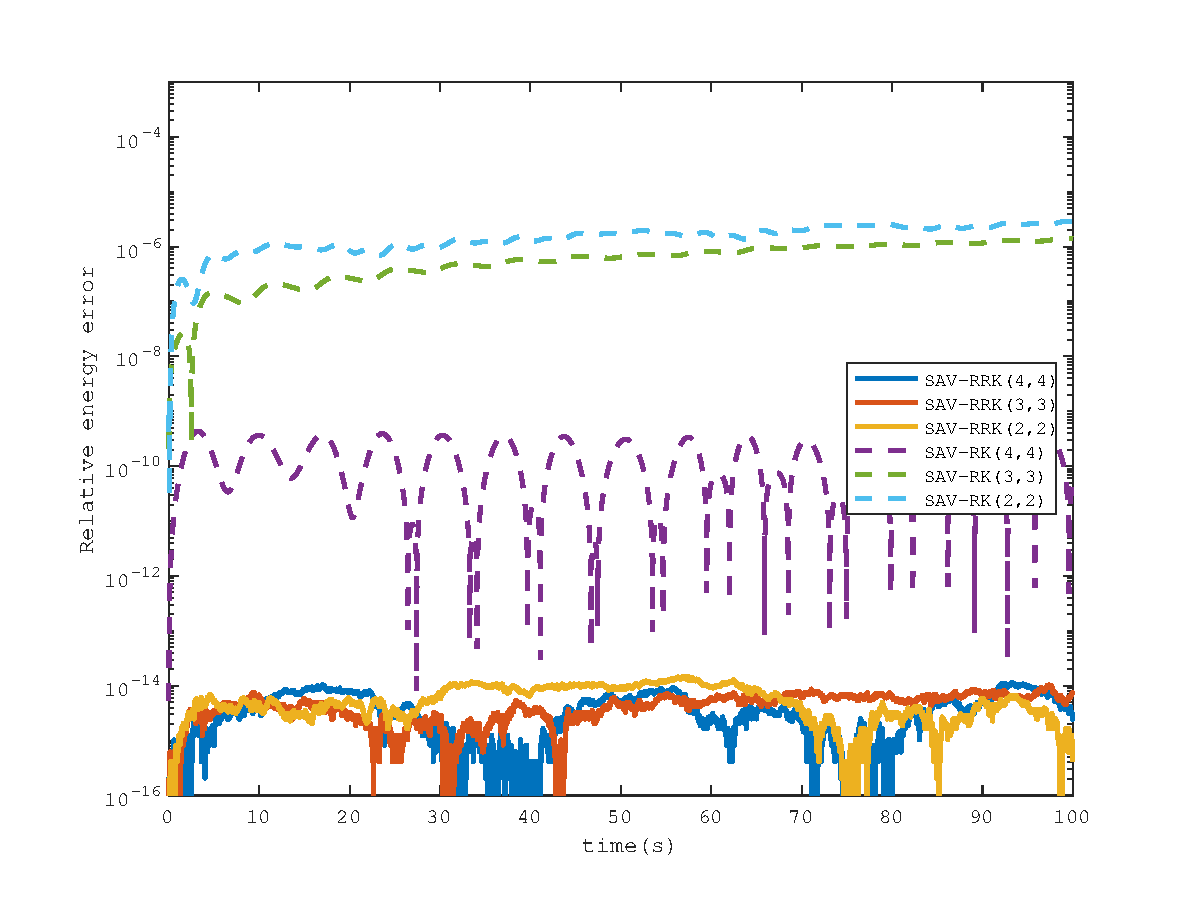
\includegraphics[width=0.5\textwidth]{./figure/exp4_energy3.eps}
%\centerline{($b$) Spatial accuracy with $\tau = 10^{-3}.$}
}\subfigure[$\alpha,\beta=1.6$]{ \centering
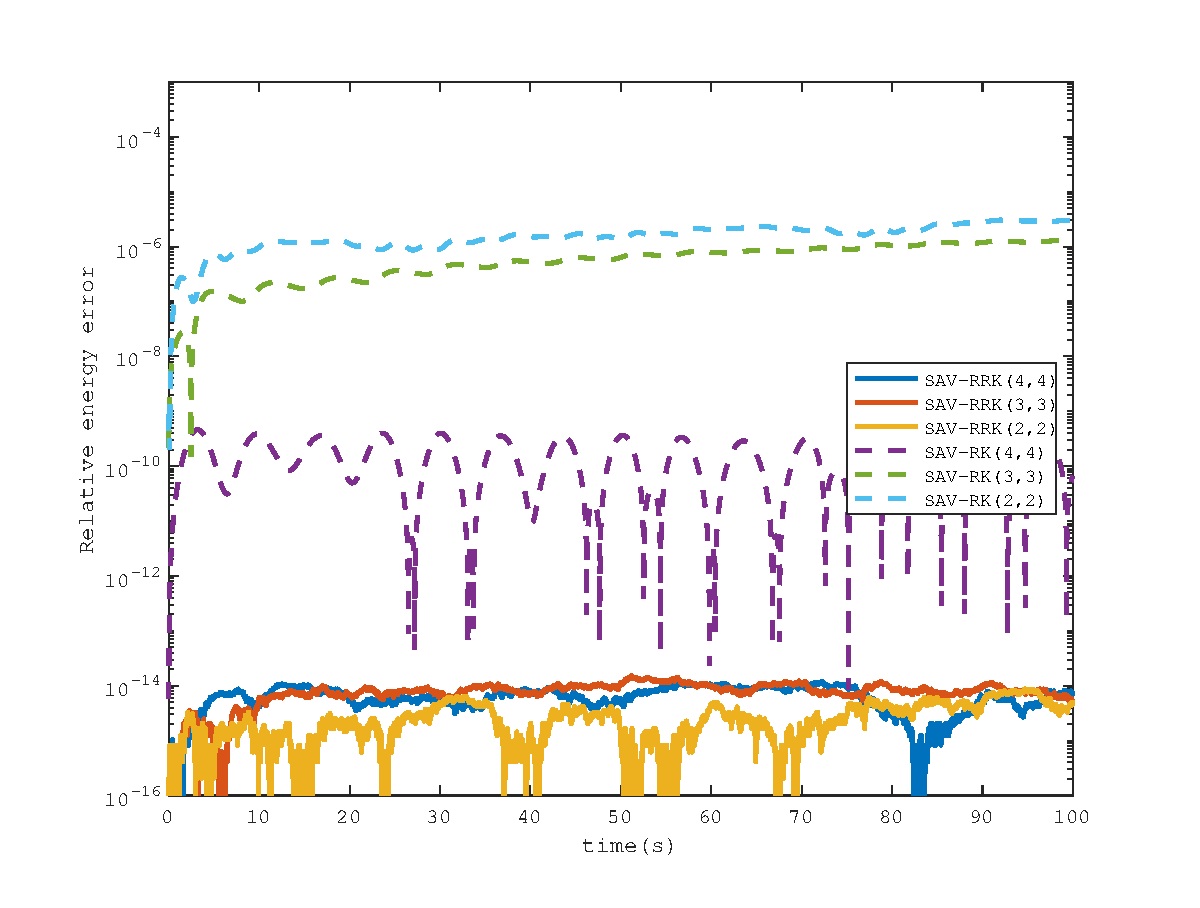
\includegraphics[width=0.5\textwidth]{./figure/exp4_energy6.eps}
%\centerline{($a$) Temporal accuracy with $N=128.$}
}\\
\subfigure[$\alpha,\beta=1.9$]{ \centering
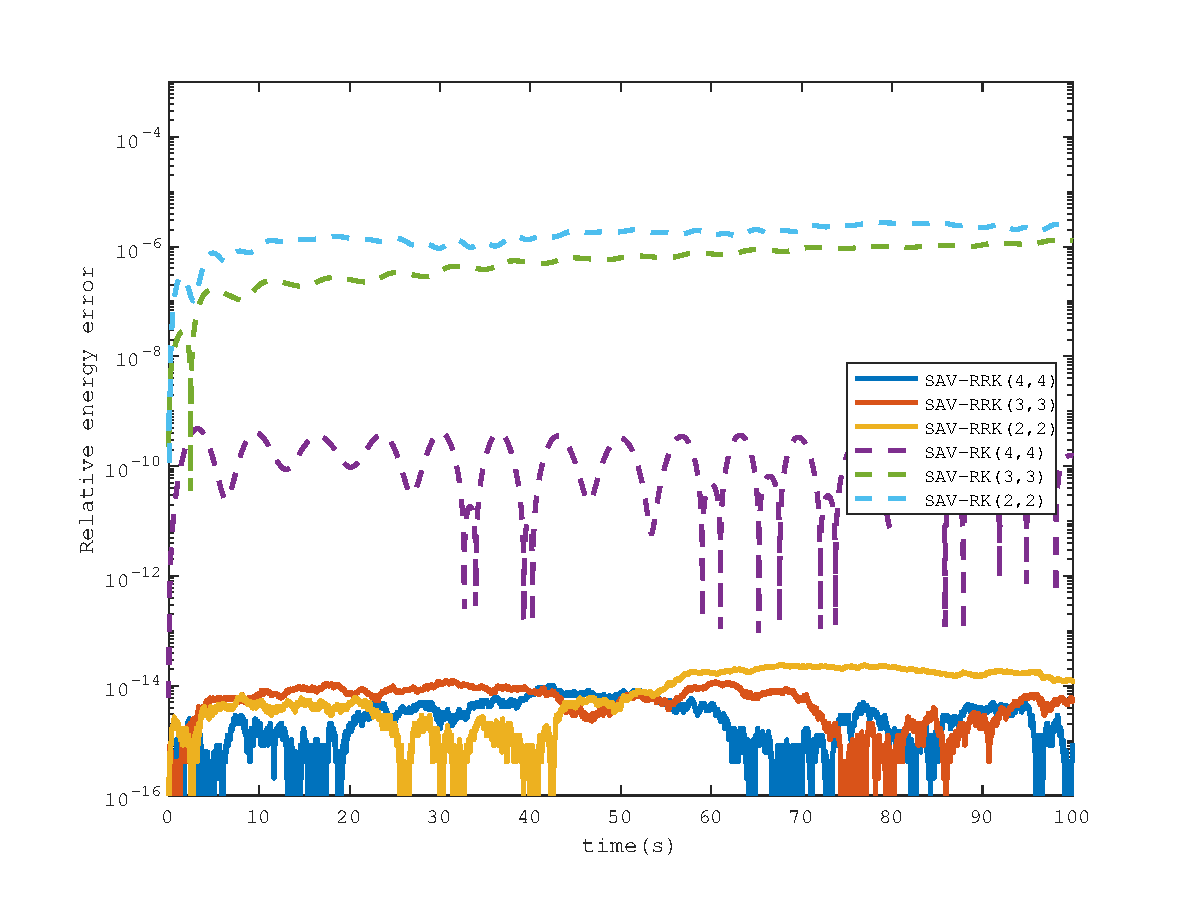
\includegraphics[width=0.5\textwidth]{./figure/exp4_energy9.eps}
%\centerline{($b$) Spatial accuracy with $\tau = 10^{-3}.$}
}\subfigure[$\alpha,\beta=2$]{ \centering
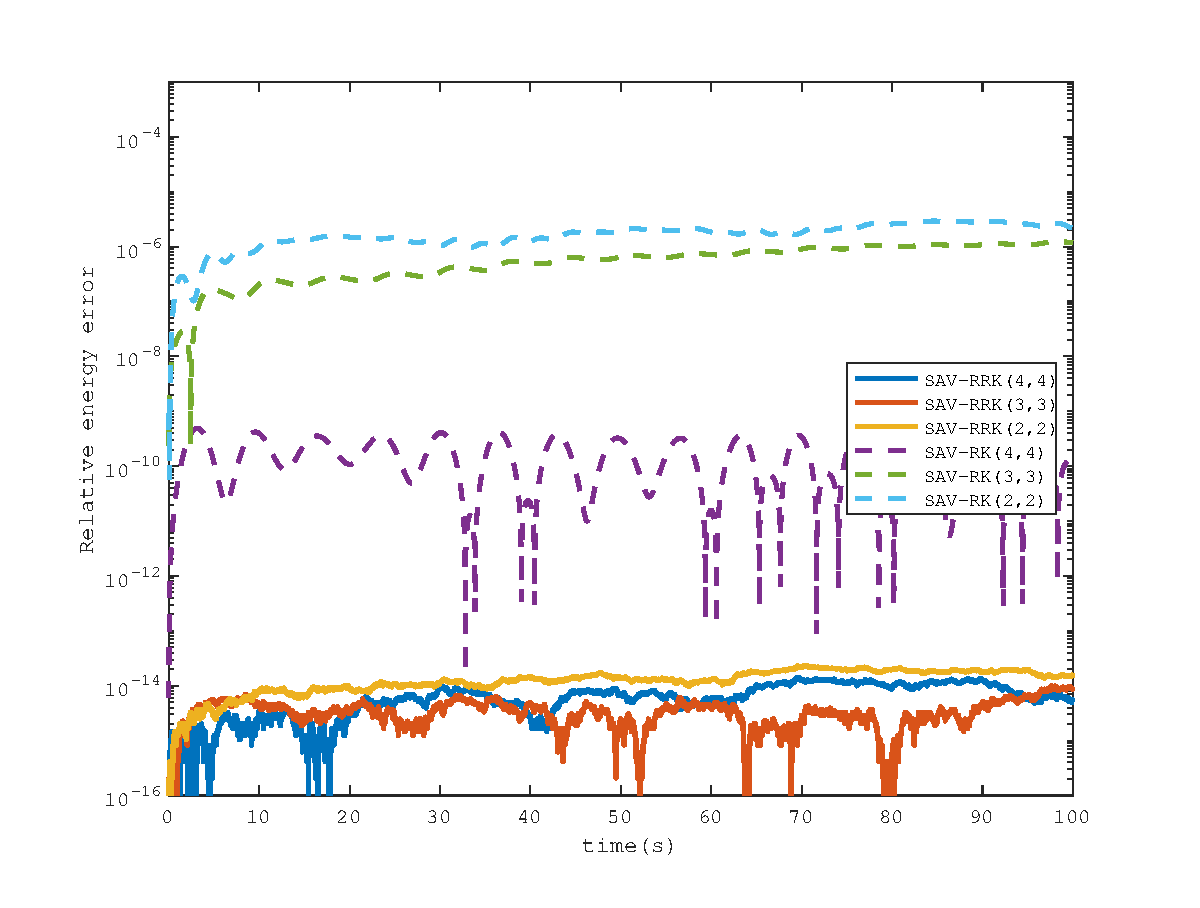
\includegraphics[width=0.5\textwidth]{./figure/exp4_energy2.eps}
%\centerline{($a$) Temporal accuracy with $N=128.$}
}\caption{ Relative errors of energy with $N=4, \tau=0.01$ for different $\alpha$ in Example \ref{ex:4}.}
\label{fig:3-5}
\end{center}
\end{figure}
	
\section{Conclusions}\label{Section 7}
In this paper, we present a new approach to develop high-order explicit energy-conserving numerical methods
for the fractional nonlinear Schr{\"o}dinger wave equations in two dimensions. The approach is proposed based on
the recently introduced scalar auxiliary variable approach and the relaxation Runge-Kutta methods. The conservation
properties of the proposed schemes are supported by theoretical analysis and numerical results.
More numerical results show that the proposed methods are also effective for other similar fractional conservative
problems, such as the nonlinear fractional wave equation and the fractional Klein-Gordon-Schr{\"o}dinger equation, etc.
%{\color{purple}{It is noteworthy that the observed phenomenon of the even-order IDT method potentially exhibiting a higher order, as suggested in other relevant literature, has not been observed in our two-dimensional calculation example. This discovery is novel, yet it remains an open question.}}

\section*{Acknowledgements}
% This work is supported by the Sichuan Science and Technology Program (Grants No. 2020YJ0110, No. 2022JDTD0019), the National Natural Science Foundation of China (Grant No. 11801389)  and the Laurent Mathematics Center of Sichuan Normal University and National-Local Joint Engineering Laboratory of System Credibility Automatic Verification (Grant No. ZD20220105).
This work is supported by the Sichuan Science and Technology Program (No. 2022JDTD0019) and the Laurent Mathematics Center of Sichuan Normal University and National-Local Joint Engineering Laboratory of System Credibility Automatic Verification (Grant No. ZD20220105).	
	%% The Appendices part is started with the command \appendix;
	%% appendix sections are then done as normal sections
% \appendix
	
		
	
%\label{}

%% If you have bibdatabase file and want bibtex to generate the
%% bibitems, please use
% \section*{References}
\begin{thebibliography}{10}
%	\expandafter\ifx\csname url\endcsname\relax
%	  \def\url#1{\texttt{#1}}\fi
%	\expandafter\ifx\csname urlprefix\endcsname\relax\def\urlprefix{URL }\fi
%	\expandafter\ifx\csname href\endcsname\relax
%	  \def\href#1#2{#2} \def\path#1{#1}\fi
	
	\bibitem{caffarelliExtensionProblemRelated2007}
	L.~Caffarelli, L.~Silvestre, An
	  Extension Problem Related to the Fractional Laplacian, Comm. Partial
	  Differential Equations 32~(8) (2007) 1245--1260.

	\bibitem{zhangConservativeNumericalScheme2003}
	L.~Zhang, Q.~Chang, A conservative numerical scheme for a class of nonlinear Schr\"odinger
	  equation with wave operator, Appl. Math. Comput. 145~(2) (2003) 603--612.

	\bibitem{baoUniformErrorEstimates2012}
	 W.~Bao, Y.~Cai, Uniform
	  Error Estimates of Finite Difference Methods for the Nonlinear
	  Schr\"odinger Equation with Wave Operator, SIAM J. Numer. Anal. 50(2) (2012) 492-521.

	\bibitem{chengSeveralConservativeCompact2018}
	X.~Cheng, F.~Wu, Several conservative compact schemes for a class of nonlinear Schr\"odinger
	  equations with wave operator, Bound. Value Probl. 2018~(1) (2018) 40.
	
	\bibitem{brugnanoClassEnergyconservingHamiltonian2018}
	L.~Brugnano, C.~Zhang, D.~Li, A class of energy-conserving Hamiltonian boundary value methods for nonlinear
	  Schr\"odinger equation with wave operator, Commun. Nonlinear Sci. Numer. Simul. 60 (2018) 33--49.

	\bibitem{colinSemidiscretizationTimeNonlinear1998}
	T.~Colin, P.~Fabrie, Semidiscretization in time for nonlinear Schr\"odinger-waves equations, Discrete Contin.
	  Dynam. Systems 4~(4) (1998) 671--690.
	
	\bibitem{ranLinearlyImplicitConservative2016}
	M.~Ran, C.~Zhang, A linearly implicit conservative scheme for the fractional nonlinear
	  Schr\"odinger equation with wave operator, Int. J. Comput. Math. 93~(7)(2016) 1103--1118.

	\bibitem{liFastEnergyConserving2018}
	M.~Li, Y.-L. Zhao, A fast energy conserving finite element method for the nonlinear fractional
	  Schr\"odinger equation with wave operator, Appl. Math. Comput. 338 (2018) 758--773.

	\bibitem{chengConvergenceEnergyconservingScheme2022}
	X.~Cheng, H.~Qin, J.~Zhang, Convergence of an energy-conserving scheme for nonlinear space fractional
	  Schr\"odinger equations with wave operator, J. Comput. Appl. Math. 400 (2022) 113762.

	\bibitem{huEfficientEnergyPreserving2022}
	D.~Hu, W.~Cai, X.-M. Gu, Y.~Wang, Efficient  energy preserving Galerkin-Legendre spectral methods for
	  fractional nonlinear Schr\"odinger equation with wave operator, Appl. Numer. Math. 172 (2022) 608--628.

	  \bibitem{zhangHighorderStructurepreservingDifference2023}
	  X.~Zhang, M.~Ran, Y.~Liu, L.~Zhang, A high-order structure-preserving difference scheme for generalized fractional
		Schr\"odinger equation with wave operator, Math Comput Simulation 210(2023) 532--546.

	\bibitem{ketchesonRelaxationRungeKutta2019}
	D.~I. Ketcheson, Relaxation Runge-Kutta Methods: Conservation and Stability for Inner-Product Norms,
       SIAM J. Numer. Anal. 57~(6) (2019) 2850--2870.

	\bibitem{ranochaRelaxationRungeKutta2020}
	H.~Ranocha, M.~Sayyari, L.~Dalcin, M.~Parsani, D.~I. Ketcheson,
	  Relaxation Runge-Kutta Methods: Fully Discrete Explicit Entropy-Stable Schemes
	  for the Compressible Euler and Navier--Stokes Equations, SIAM J.
	  Sci. Comput. 42~(2) (2020) A612--A638.

	\bibitem{yangLinearUnconditionallyEnergy2017}
	X.~Yang, L.~Ju, Linear and unconditionally energy stable schemes for the binary fluid-urfactant phase field model,
      Comput. Methods Appl. Mech. Eng. 318 (2017) 1005--1029.

	\bibitem{yangEfficientLinearSchemes2017}
	X.~Yang, L.~Ju, Efficient linear schemes with unconditional energy stability for the phase field
	  elastic bending energy model, Comput. Methods Appl. Mech. Eng. 315 (2017) 691--712.

	  \bibitem{hairerRungeKuttaMethods2015}
    E.~Hairer, G.~Wanner, Runge-Kutta  Methods, Explicit, Implicit, Encycl. Appl. Comput. Math., 2015, pp. 1282--1285.

	\bibitem{liImplicitexplicitRelaxationRungeKutta2022}
	D.~Li, X.~Li, Z.~Zhang, Implicit-explicit relaxation Runge-Kutta methods: Construction, analysis and applications
	  to PDEs, Math. Comp. 92~(339) (2022) 117--146.

	\bibitem{ranochaGeneralRelaxationMethods2020}
	H.~Ranocha, L.~L{\'o}czi, D.~I. Ketcheson, General relaxation methods
	  for initial-value problems with application to multistep schemes, Numer.
	  Math. 146~(4) (2020) 875--906.

	\bibitem{wangConservativeLinearizedDifference2015}
	P.~Wang, C.~Huang, A conservative linearized difference scheme for the nonlinear fractional
	  Schr\"odinger equation, Numer. Algorithms 69~(3) (2015) 625--641.

	\bibitem{wangUnconditionalEnergyDissipation2021}
	N.~Wang, M.~Li, C.~Huang, Unconditional Energy Dissipation and Error Estimates of the SAV Fourier Spectral
	  Method for Nonlinear fractional  wave equation, J. Sci. Comput. 88~(1) (2021) 19.

	\bibitem{fuStructurepreservingAlgorithmsTwodimensional2020}
	Y.~Fu, W.~Cai, Y.~Wang, Structure-preserving
	  algorithms for the two-dimensional fractional Klein-Gordon-Schr\"odinger
	  equation, Appl. Numer. Math. 156 (2020) 77--93.

	\end{thebibliography}
	
	

% \bibliographystyle{elsarticle-num}
% \bibliography{/Users/dasha/Zotero/BetterBibTeX/mylibrary.bib}

\end{document}
